%% ----------------------------------------------------------------------------
% BIWI SA/MA thesis template
%
% Created 09/29/2006 by Andreas Ess
% Extended 13/02/2009 by Jan Lesniak - jlesniak@vision.ee.ethz.ch
%% ----------------------------------------------------------------------------
\newpage
\chapter{Semi-supervised image segmentation}
The philosophy behind semi-supervised learning is to propagate label information from labeled to unlabeled data. Image segmentation can be seen as a classification problem which consists of assigning a class label to each pixel. For our task of binary segmentation, this means classifying each pixel as foreground or background. For our task of image segmentation, we make use of partial annotations as \textit{scribbles}. Scribbles are pixels in image annotated by experts as foreground or background. We use example-based methods to learn from these scribbles annotated by experts. In contrast to having different images for training and testing, we use same image for training and testing as the samples used for training are pixels and not images.

\section{Random Forest}
In this section, we make use of random forest (RF) as the semi-supervised learning algorithm. The advantages and details of using RF can be found in Eugster. For training RF, we compute set of features in Python. We compute different features ranging from simple Sobel edge detectors to higher level Gabor filters. The choice of features was made according to WEKA \cite{weka} toolset of FIJI \cite{fiji} plugin. These are set of 2D features and perform well for medical images. We compute the different type of features for a range of sigmas, which gives 69 feature maps for a single image. In the thesis by Eugster \cite{dominic}, we can find details and effect of feature selection for training Random forests. As shown in figure 3.1, we can observe that for given annotation budget, the segmentation measure does not change significantly for more than 30 trees and for more than 20 features. Therefore, for all experiments using RF, we use 20 best features and 30 trees for training. In this thesis, we focus on how to get best results for given annotation budget and thus, use fixed number of features and trees to generate masks.  We try to answer the question of where to scribble and how to make the best use of our annotation budget and time.

\begin{figure}[h!] \label{fig:rf_complex}
\begin{tabular}{cc}
 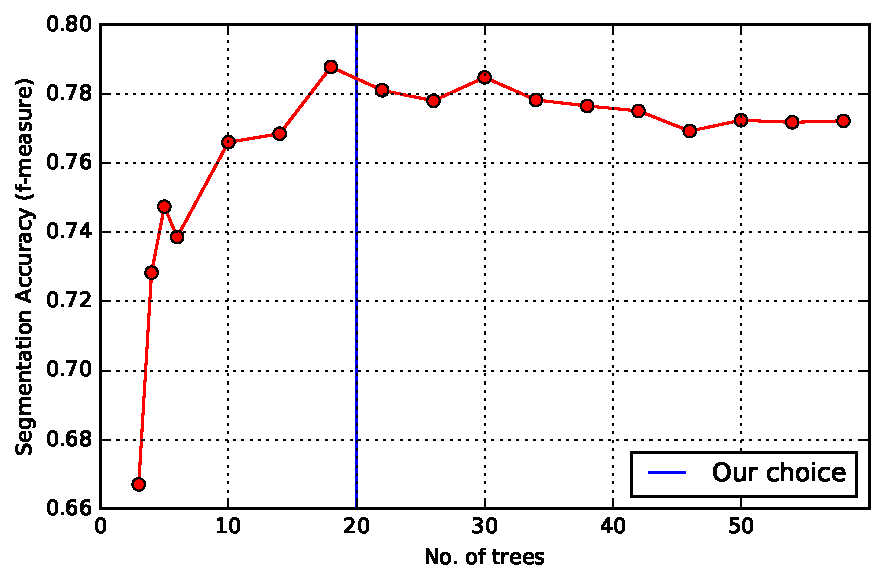
\includegraphics[width=0.5\linewidth]{figures/diff_features.pdf} & 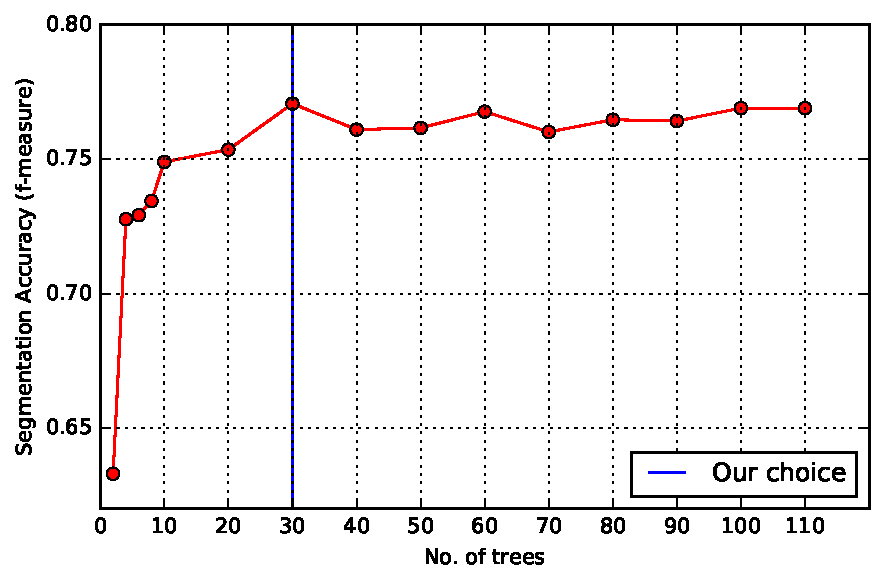
\includegraphics[width=0.5\linewidth]{figures/diff_trees.pdf} \\
  (a)  & (b) \\
\end{tabular}
\caption{Plot of segmentation measure vs changing complexity of RF: (a) with features, (b) with trees}
\end{figure}


\subsection{Where to scribble?}
In general, we believe that the more training data we provide, more we can improve the results. Does this hold for partial annotation such as scribbles? If we go on increasing the pixels annotated arbitrarily, will it improve the segmentation mask or we have to use our labeling effort intelligently to improve results? We conducted an experiment by dividing our set of foreground and background scribbles into 2 classes: easy and hard. We classified scribbles as "easy" and "hard" depending on the effort required to annotate these pixels. For example, pixels are difficult to annotate near the boundary of foreground and background, and we classify these pixels as "hard", as shown in figure 3.2. We manually scribbled image for both "easy" and "hard" subclasses. Then, we trained and tested RF on one image by increasing percentage of scribbles belonging to "easy" foreground and background class. After we have used all scribbles belonging to "easy" class, we added scribbles from "hard" class for both foreground and background. The increment was done w.r.t. the total amount of scribbles we are having and also, for a higher percentage of added scribbles, we maintained a ratio between foreground and background pixels. The result can be observed in figure 3.3(a). \par


\begin{figure}[h!] \label{fig:scribbles}
\begin{tabular}{cc}
 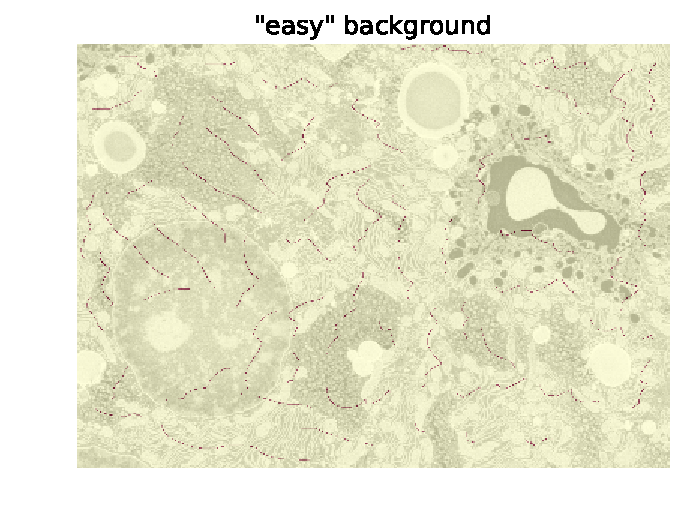
\includegraphics[width=0.5\linewidth]{figures/easy_bg.pdf} & 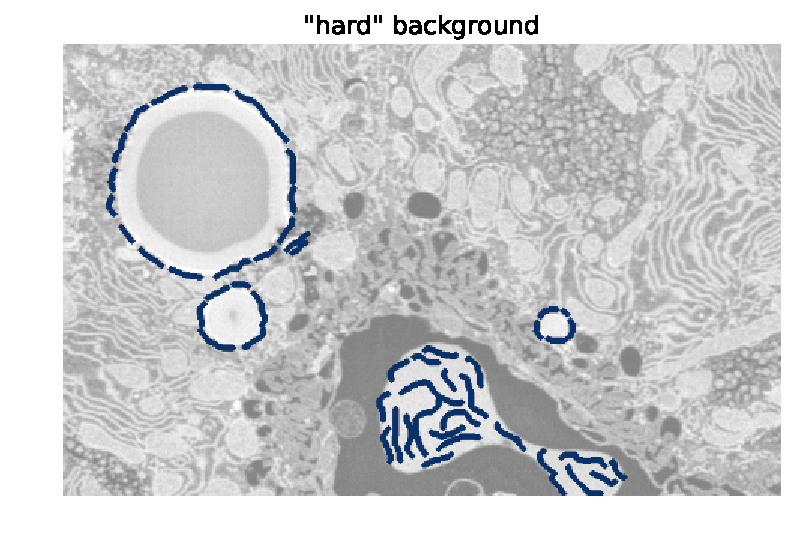
\includegraphics[width=0.5\linewidth]{figures/hard_bg.pdf} \\
 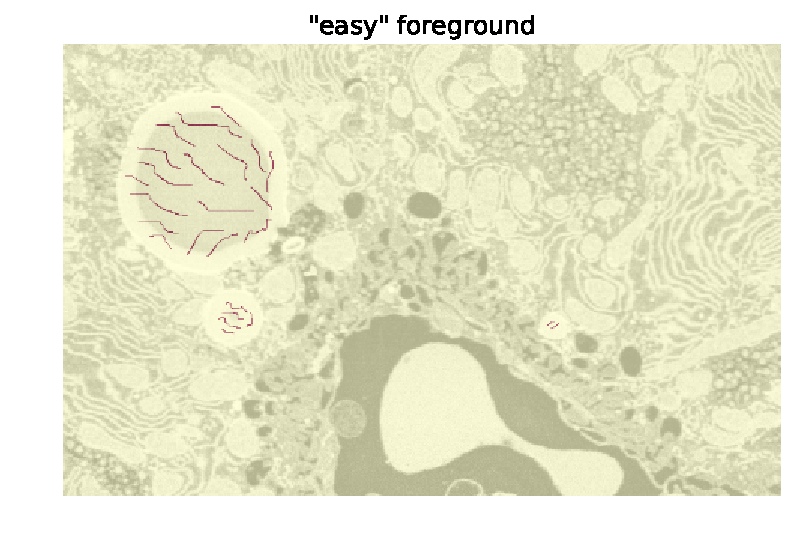
\includegraphics[width=0.5\linewidth]{figures/easy_fg.pdf} & 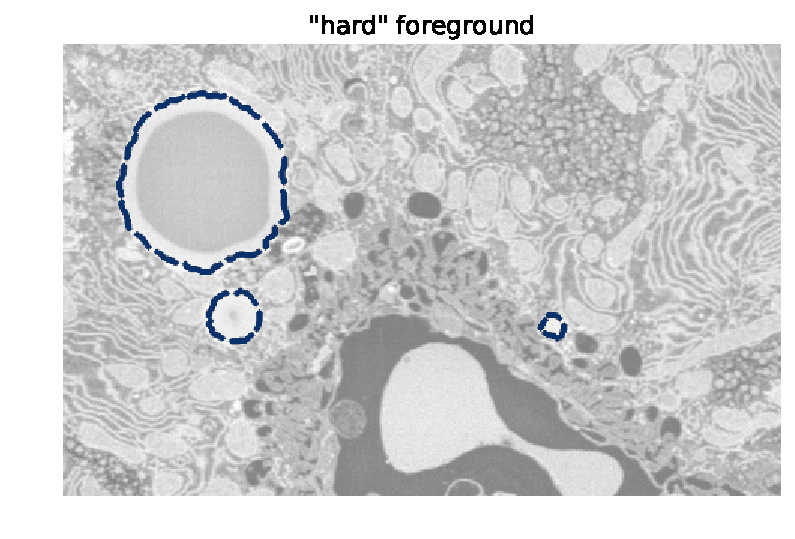
\includegraphics[width=0.5\linewidth]{figures/hard_fg.pdf} \\ 
\end{tabular}
\caption{Manual scribbles in "easy" and "hard" classes}
\end{figure}


\begin{figure}[h!] \label{fig:easy_hard1}
 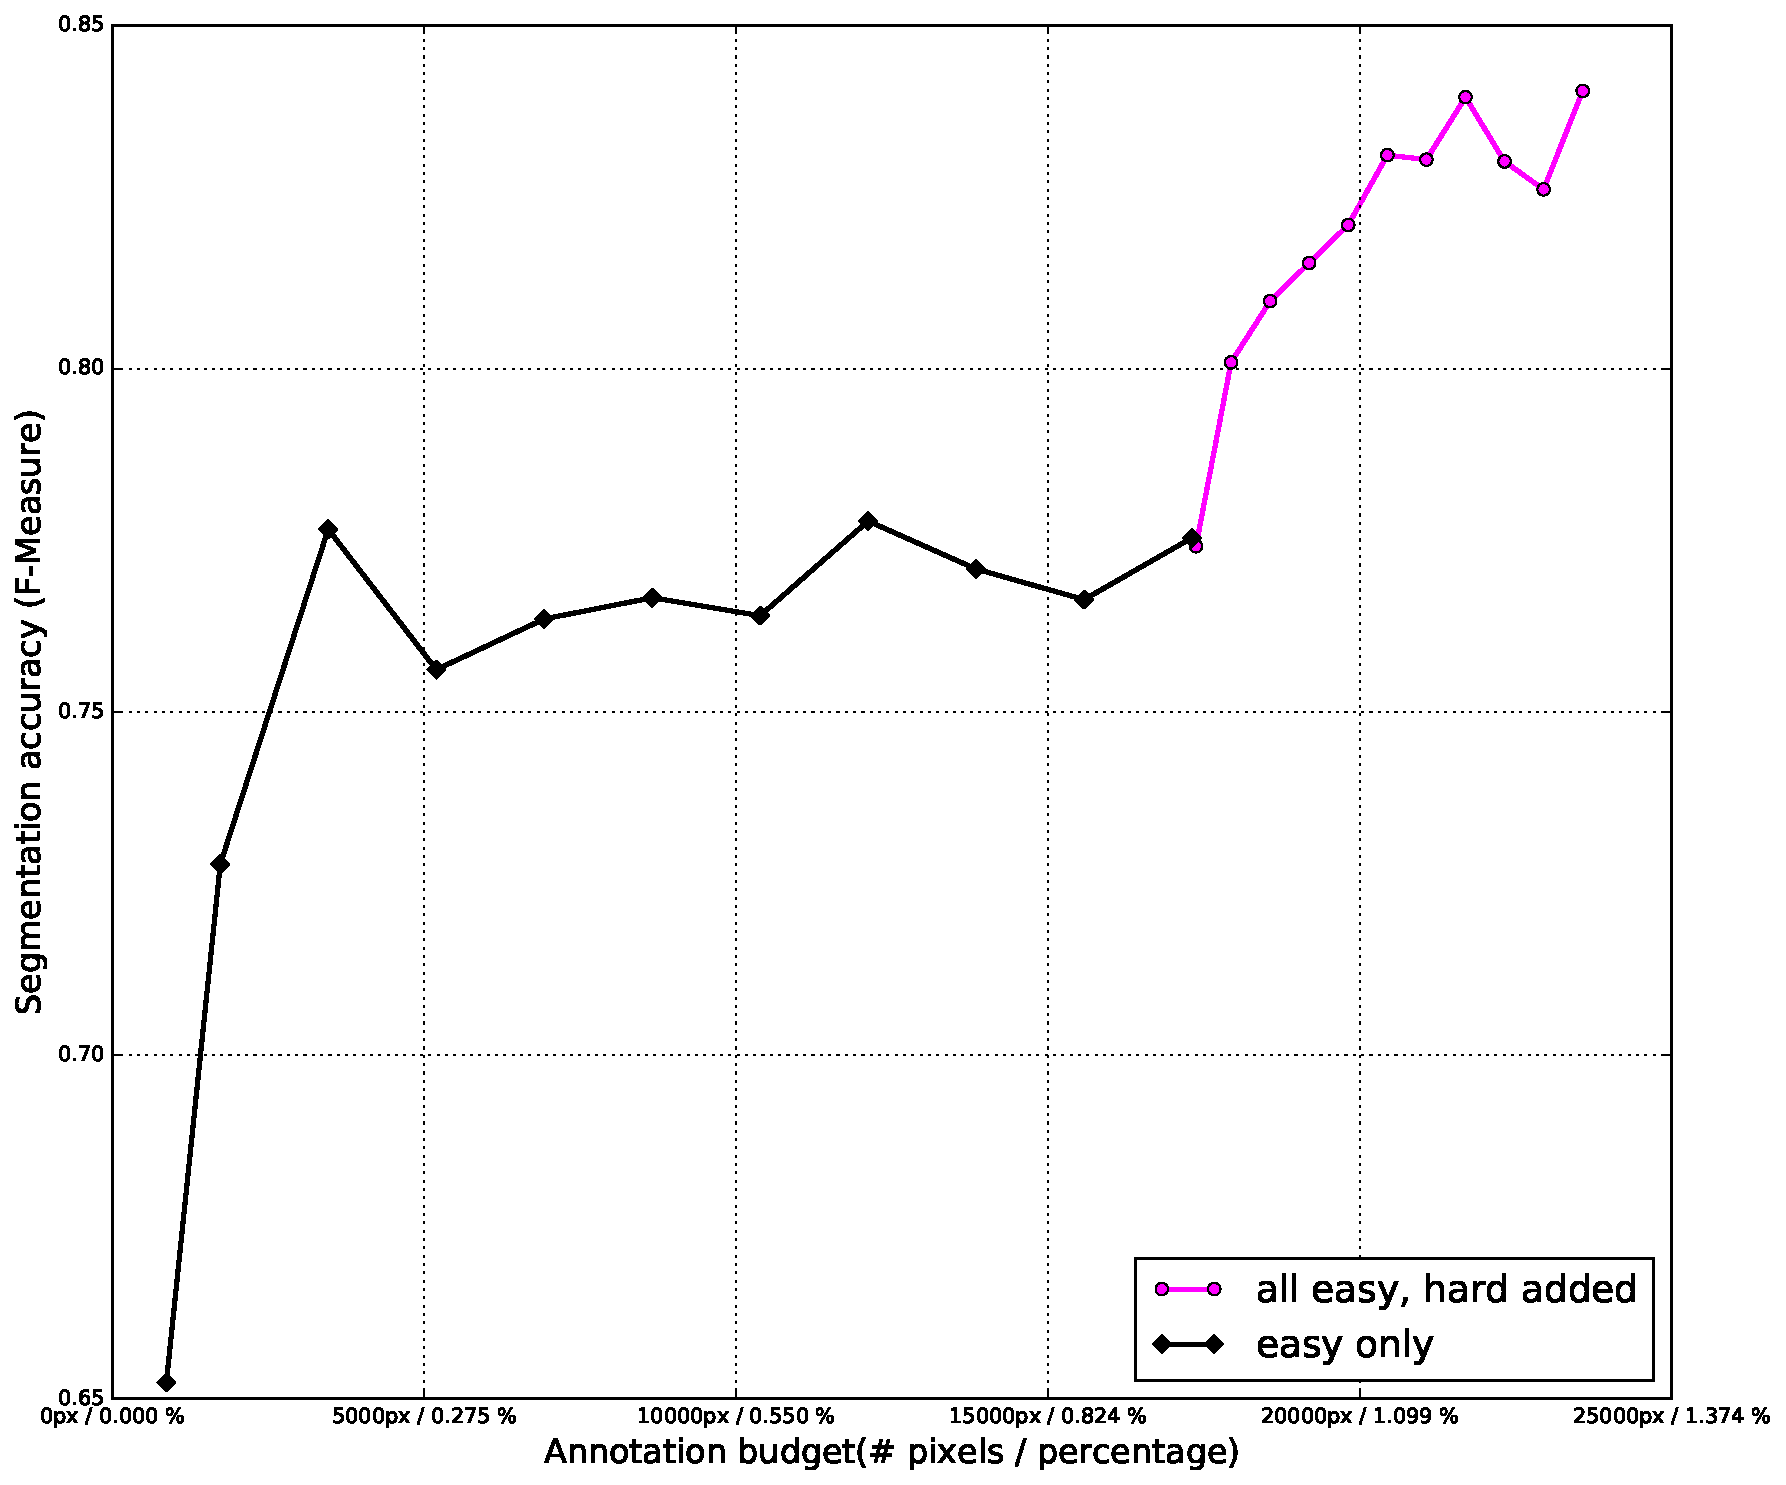
\includegraphics[width=1.0\linewidth]{figures/rf_easy_hard.pdf}
\caption{Plot of segmentation measure vs annotation budget. The black curve shows change in segmentation measure with increment of scribbles from "easy" class. Other curves and show change in segmentation measure with increment of scribbles from "hard" class, starting with different fixed amount of "easy" class.}
\end{figure}


In figure 3.3(a), we can observe that after a total of 3000 pixels selected from "easy" foreground and background, the segmentation measure does not change significantly. An improvement can be observed, once we started adding "hard" scribbles after all "easy" scribbles were used. This shows that the best results can be obtained by adding "hard" scribbles after addition of a certain percentage of "easy" scribbles. Looking at the plot, one might think to start adding the "hard" scribbles after 3000 "easy" scribbles. We tried this and results can be observed in figure 3.3(b). \par

In figure 3.3(b), as we started adding "hard" scribbles on top of 10\% (3000 pixels) of scribbles selected from "easy" scribbles, instead of observing a rise with additional scribbles, we observed a fall in performance (dark blue plot in figure 3.3(b)). This may be due to lack of enough "easy" scribbles and RF starts training its trees to focus more on "hard" scribbles. We tried a similar experiment with the different amount of "easy" scribbles to start with. We started seeing a significant improvement when we utilized with 70\% of all "easy" scribbles to train RF. We were able to achieve f-measure score of 0.83 in comparison of 0.84 achieved with 100\% usage of "easy" scribbles (See green and pink plot in figure 3.3(b)). Thus, the question arises how to decide the point of addition of "hard" scribbles. 

\subsection{Iterative semi-interactive approach}
In the previous section, we showed the need of using our annotation budget intelligently to get the best performance. But, we observed the problem of deciding on how many "easy" and "hard" scribbles are needed to achieve best results. For our problem, we divided the scribbles as "easy" and "hard" according to labeling effort, but this division for scribbles may not be same from point of view of the Random forest. Apriori, we don't know which pixels will be difficult for the Random forest to classify correctly. The above mentioned two problems can be solved by annotating pixels iteratively to improve results, at least once to understand which pixels are difficult for RF to classify. We show the improvement in the result by doing one iteration in figure 3.4. We can observe that the scribbles are very few to produce a good result. Still, we can observe improvement in f-measure from 0.745 to 0.749 for increasing the annotation budget from 7500 pixels to 10900. Although the increment looks insignificant, but we can observe the difference in the large vesicle in left-top corner of the image.
\begin{figure}[h!] \label{fig:semi-rf}
 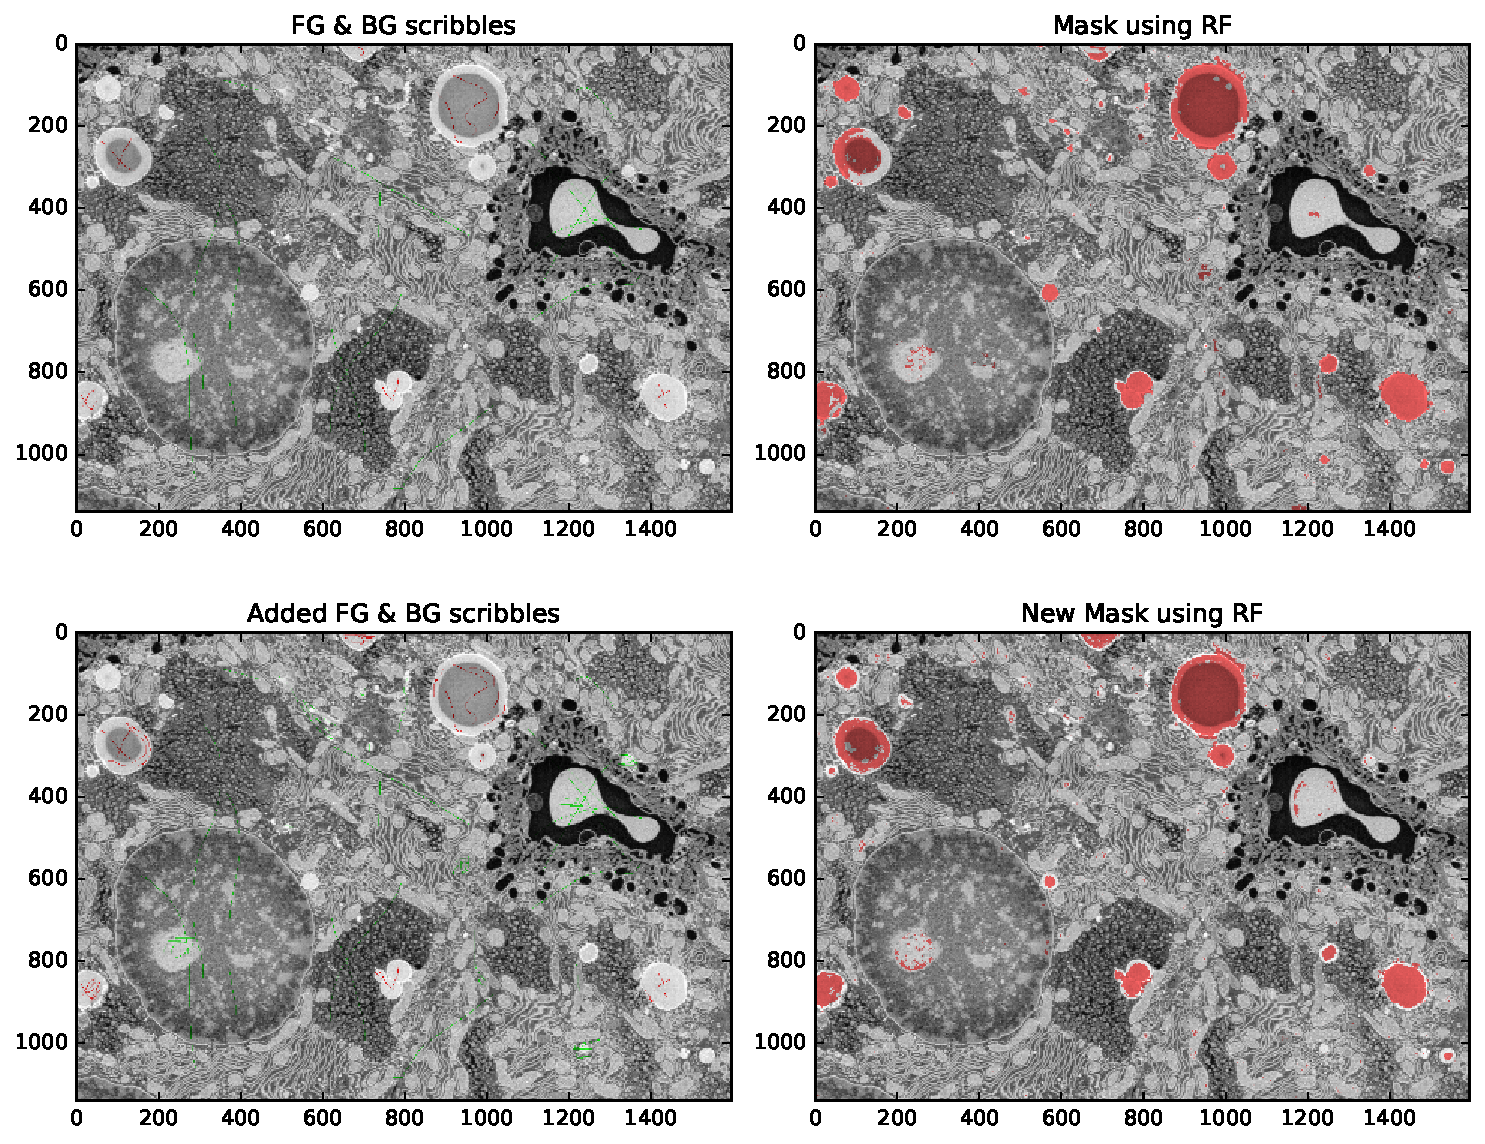
\includegraphics[width=1.0\linewidth]{figures/semi_inter_rf.pdf}
\caption{Semi-interactive segmentaion with one iteration}
\end{figure}

\subsection{Uncertainity of classifier}
The use of iterative semi-interactivity gives the best result for given annotation budget, but the output of RF is noisy and uncertain. The uncertainty lies in the inability to classify maximum of pixels as foreground and background, as shown in figure 3.5(a). The histogram shows the distribution of probability values for the complete image. It can be seen that a large number of pixels are not given a probability of 0 (background) or 1 (foreground). In figure 3.5(b), we can observe varying results for different threshold applied on output from RF. RF acts as a classifier and classifies each pixel but we need to group these pixels into objects for segmentation. In this thesis, we make use of prior information to compensate for the lack of enough annotated data and for the uncertainty of classifier.

\begin{figure}[h!] \label{fig:uncertain}
\begin{tabular}{cc}
 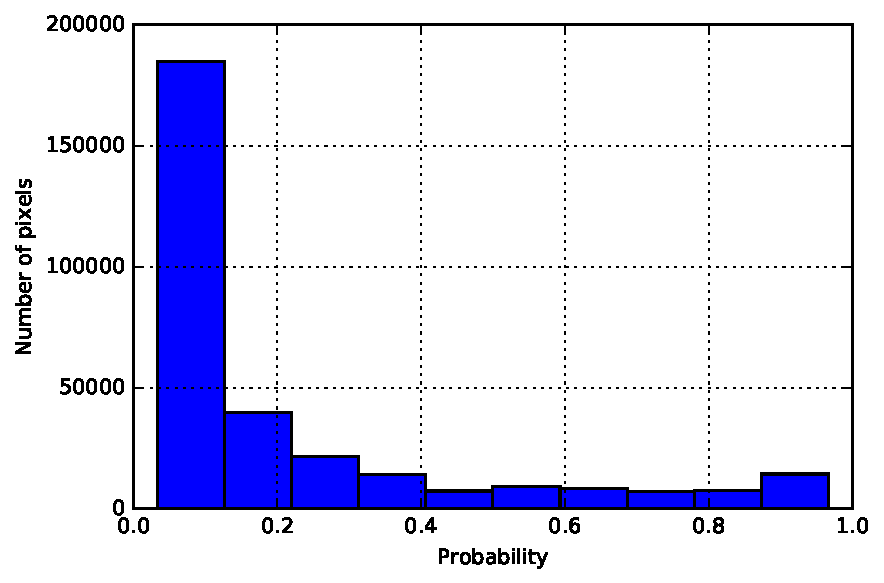
\includegraphics[width=0.5\linewidth]{figures/hist.pdf} & 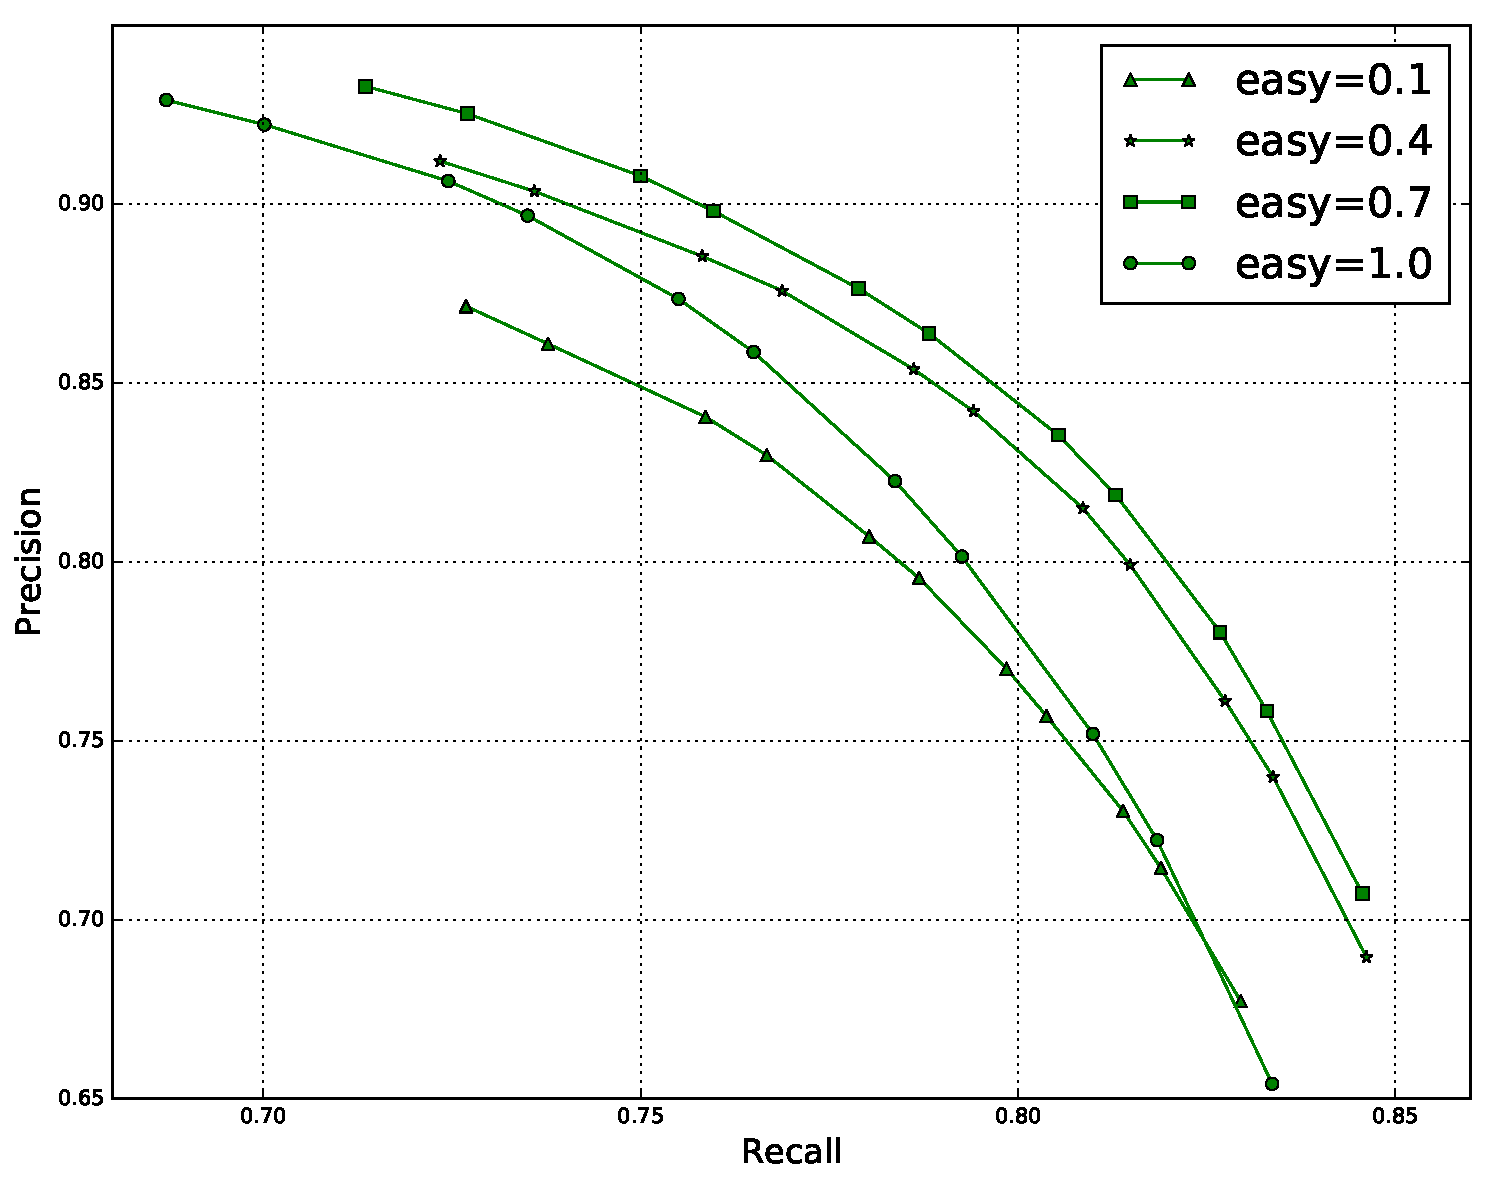
\includegraphics[width=0.5\linewidth]{figures/pr_curve.pdf} \\
  (a)  & (b) \\
\end{tabular}
\caption{(a) Histogram of probabilities. (b) Precision-recall curve for varying thresholded RF mask. Different curves for different annotation budget}
\end{figure}

\section{Bayesian Formulation}
To make use of prior, we model our image segmentation problem as a Bayesian inference problem. Let us cosider an observed image, $\mat{I}$ and labeled or segmented ground truth, $\mat{M}$, the joint probabilty can be defined as:
\begin{equation*}
\p(\mat{I}, \mat{M}) = \p(\mat{M}) \p(\mat{I}|\mat{M}) \eqcont
\end{equation*}
and applying Bayes theorem,
\begin{align*}
\p(\mat{M}|\mat{I}) \, & = \frac{\p(\mat{M}) \p(\mat{I}|\mat{M})}{\p(\mat{I})} \\
						& \alpha \, {\p(\mat{M}) \p(\mat{I}|\mat{M})}
\end{align*}
The left hand side is the probability of obtaining segmentation mask, $\mat{M}$ given the image $\mat{I}$, is called the posterior probability. $\p(\mat{M})$ is the prior probability of mask, $\mat{M}$. The Maximum a posteriori (MAP) estimate, $\mat{M^*}$ can be calculated as follow:
\begin{equation}
\mat{M^*} = \arg\max_{\mat{M}}({\p(\mat{M}) \p(\mat{I}|\mat{M})}) \eqend
\end{equation}

The above problem can as well be stated as an energy minimization problem by
writing Equation 3.1 in terms of energy by taking negative log-likelihood:
\begin{align*}
\funop{E}(\mat{M}) &=\, - \, \log(\p(\mat{I}, \mat{M})) \\
&= -\, \log(\p(\mat{I}|\mat{M})) - \log(\p(\mat{M})) \\
&= \funop{E_d}(\mat{I}, \mat{M}) + \funop{E_r} (\mat{M})
\end{align*}
The total energy, $\funop{E}$, that we want to minimize can be considered as linear combination of data or likelihood term, $\funop{E_d}$ and prior term (or regularization), $\funop{E_r}$. This modifies calculating MAP estimate to:
\begin{equation*}
\mat{M^*} = \arg\min_{\mat{M}}({\funop{E_d}(\mat{I}, \mat{M}) + \funop{E_r} (\mat{M})}) \eqend
\end{equation*}
To obtain MAP estimate, we need to formulate likelihood term and prior term. We formulate the prior using Total variation(TV). We can find use of different TV priors such as Wulff shapes etc. In our thesis, as the objects we need to segment are smooth and shaped like a circle, we make use of isotropic total variation, $\funop{TV}$. Also, we can try to use isotropic total variation in 2D and 3D as the data we are trying to segment is a 3D stack. For likelihood term, G. Paul et al.\cite{Paul2013} proposed an energy formulation which is not derived from a statistical model but learnt from training set. This gives the advantage of combining example-based and model-based approaches. Similar to Eugster \cite{dominic}, we formulate the likelihood term as product term of a cost function, $\funop{C}$, of soft mask, $\mat{P}$(probability of each pixel being foreground) learnt from RF and optimal mask to be estimated, $\mat{M}$. The energy minimization problems becomes:
\begin{align*}
\funop{E}(\mat{M}) &= \funop{E_d}(\mat{I}, \mat{M}) + \funop{E_r} (\mat{M}) \\
&= <\funop{C}(\mat{P}), \mat{M}> + \lambda\, \funop{TV}(\mat{M}) + \mathrm{i}_{[0,1]}(\mat{M}) \eqcont 
\end{align*}
where $\mathrm{i}_{[0,1]}(\mat{M})$ is an indicator function to ensure values of $\mat{M}$ remain in [0,1]. In addition to use of cost function, we enforce constraint of preserving the pixels annotated by experts as foreground and background in our energy minimization problem. We used an indicator function, $\mathrm{i}_{fg}(\mat{M})$, to ensure pixels in foreground scribbles have value of 1 in mask, and indicator function, $\mathrm{i}_{bg}(\mat{M})$, to ensure pixels in background scribbles have value of 0 in mask. Using discrete implementaion of TV, the final energy minimization problem is formulated as given below:
\begin{align*}
\funop{E}(\mat{M}) &= <\funop{C}(\mat{P}), \mat{M}> + \lambda\, \||\mat{D}\mat{M}|_2\|_1 + \mathrm{i}_{[0,1]}(\mat{M}) + \mathrm{i}_{fg}(\mat{M})  + \mathrm{i}_{bg}(\mat{M}) 
\end{align*}

The optimization problem is solved using Alternating Split Bregman method (ASB), as described in Eugster \cite{dominic}. The advantage of using ASB is that it splits the above problem into subproblems. Each subproblem is easy to solve and can be solved independently. The final solution to the problem is obtained by iterating updates. The details of implementation and solution can be obtained from Eugster \cite{dominic}. The results for RF with variational segmentation (with \textbf{\textit{anti-nll}} cost function described in following section) can be seen in figure 3.6. We can observe different improvement due to the use of the variational method for different regularization parameter ($\lambda$). The boost obtained from variational image processing (VIP) with best among different $\lambda$ can be seen in figure 3.7. The advantage can be seen that the boost is always positive implying that use VIP never degrades the performance of RF. In the following section, we describe and compare the use of different cost functions in Variational segmentation methods.


\begin{figure}[h!] \label{fig:rf_vipfull}
 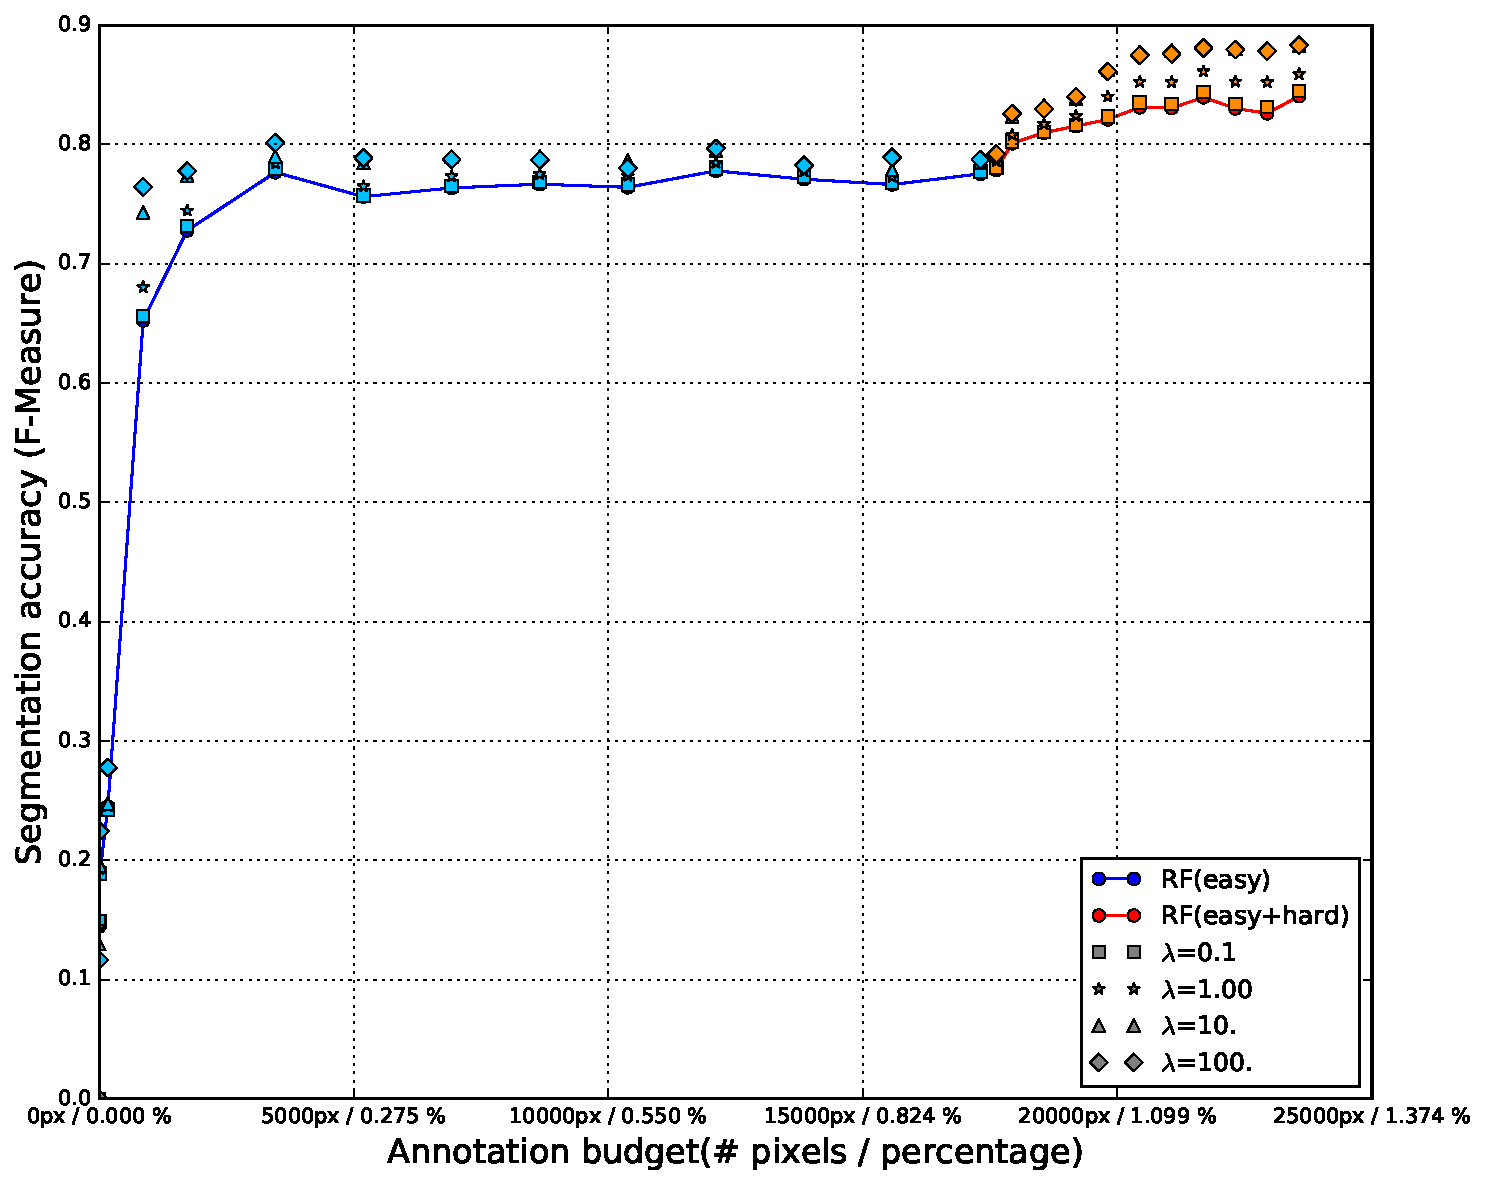
\includegraphics[width=1.0\linewidth]{figures/rf_vip_easy_hard_full.pdf}
\caption{Segmentation score with RF and prior(TV) for different annotation budget}
\end{figure}


\begin{figure}[h!] \label{fig:rf_vip}
 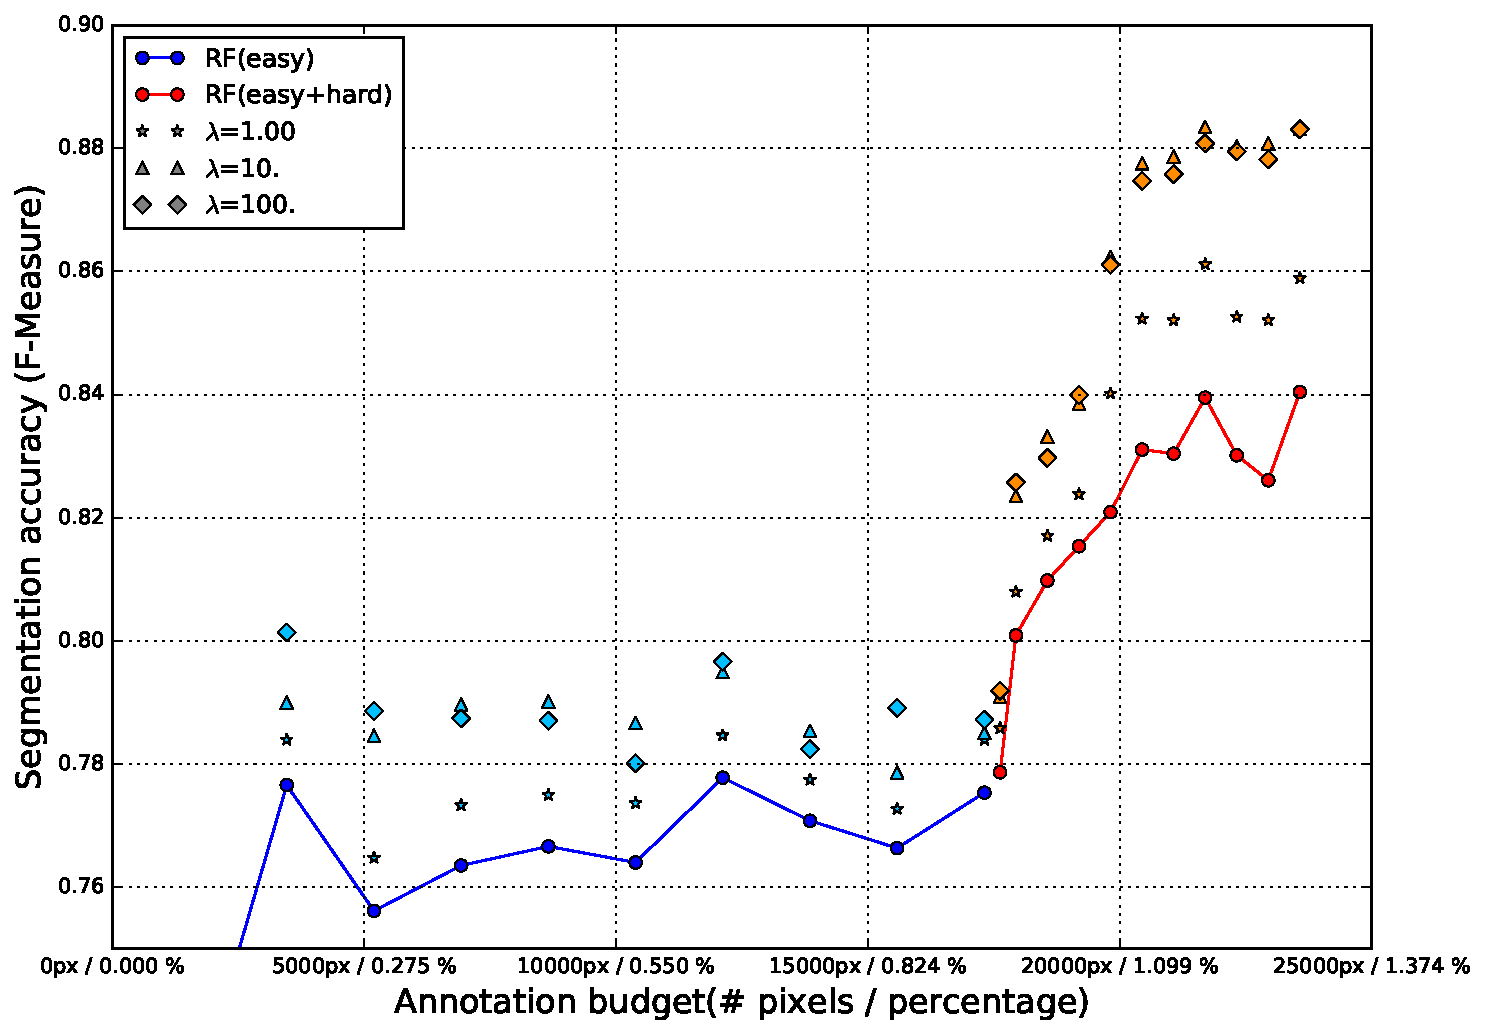
\includegraphics[width=1.0\linewidth]{figures/rf_vip_easy_then_hard.pdf}
\caption{Segmentation score with RF and prior(TV) for different annotation budget}
\end{figure}


\begin{figure}[h!] \label{fig:rf_vip1}
 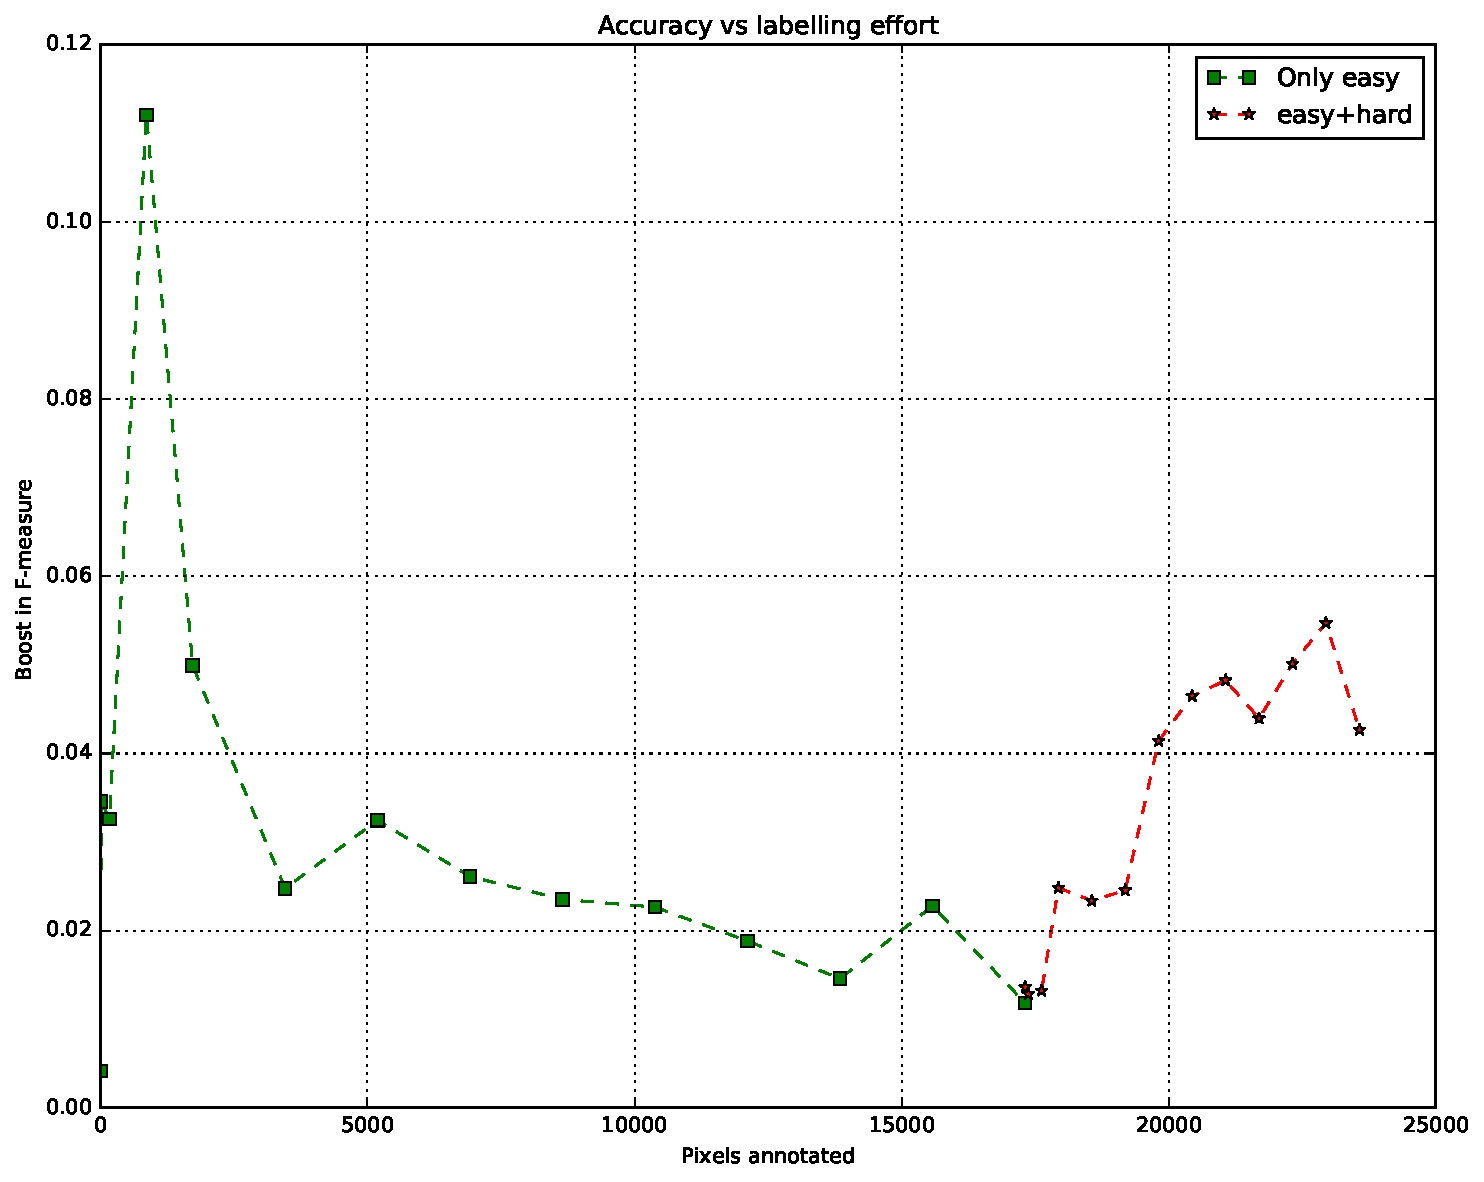
\includegraphics[width=1.0\linewidth]{figures/vip_boost.pdf}
\caption{Boost obtained with VIP over RF Segmentation score with RF and prior(TV) for different annotation budget}
\end{figure}

\subsection{Different likelihhood formulations}
In literature, people have formulated the cost function either directly using the soft mask ($\mat{P}$) obtained from RF or, some linear or non-linear function of the mask. Santner \cite{santner:2009} formulates likelihood term as linear function of mask, $\funop{C_l}$, as given below:
\begin{align*}
\funop{C_l}(\mat{P}) = -4\,(\mat{P}-0.5) \eqend
\end{align*}
We used, \textbf{\textit{anit-nll}} cost function, $\funop{C_{nll}}$, as given below:

\begin{align*}
\funop{C_{nll}}(\mat{P}) =
\begin{cases}
  0, & \text{if}\ pixel \in Scribbles  \\
  -\log \frac{\mat{P}}{1-\mat{P}}, & \text{else}
\end{cases}
\end{align*} 
For \textit{anti-nll} cost function, we need to use foreground and background constraint for pixel with probability 0 or 1 as we do for scribbles. In addition to the cost function, Santner \cite{santner:2009} mentioned use of hard constraint for pixels in foreground or background scribbles i.e. using cost of $-\infty$ for foreground scribbles and $\infty$ for background scribbles. They didn't show a way to enforce this constraint with \textit{linear} cost function. We enforced this constraint with use of indicator functions. \par
We used different amount of annotated pixels, randomly selected from ground truth and generated segmentation mask using RF and TV with different cost functions. We generated results to compare 3 cost functions: \textit{linear}, \textit{linear with constraints} and \textit{anti-nll (with constraints)}. The results can be observed in figure 3.8. The 
\textit{linear} cost function does not work well with large values of $\lambda$ and also deteriorates the mask obtained from RF. This does not happen with \textit{linear with constraints} and \textit{anti-nll}, where VIP performs always better than RF. This shows robustness of using \textit{linear with constraints} and \textit{anti-nll} cost functions.
\begin{figure}[h!] \label{fig:rf_vip1}
% \begin{tabular}{ccc}
 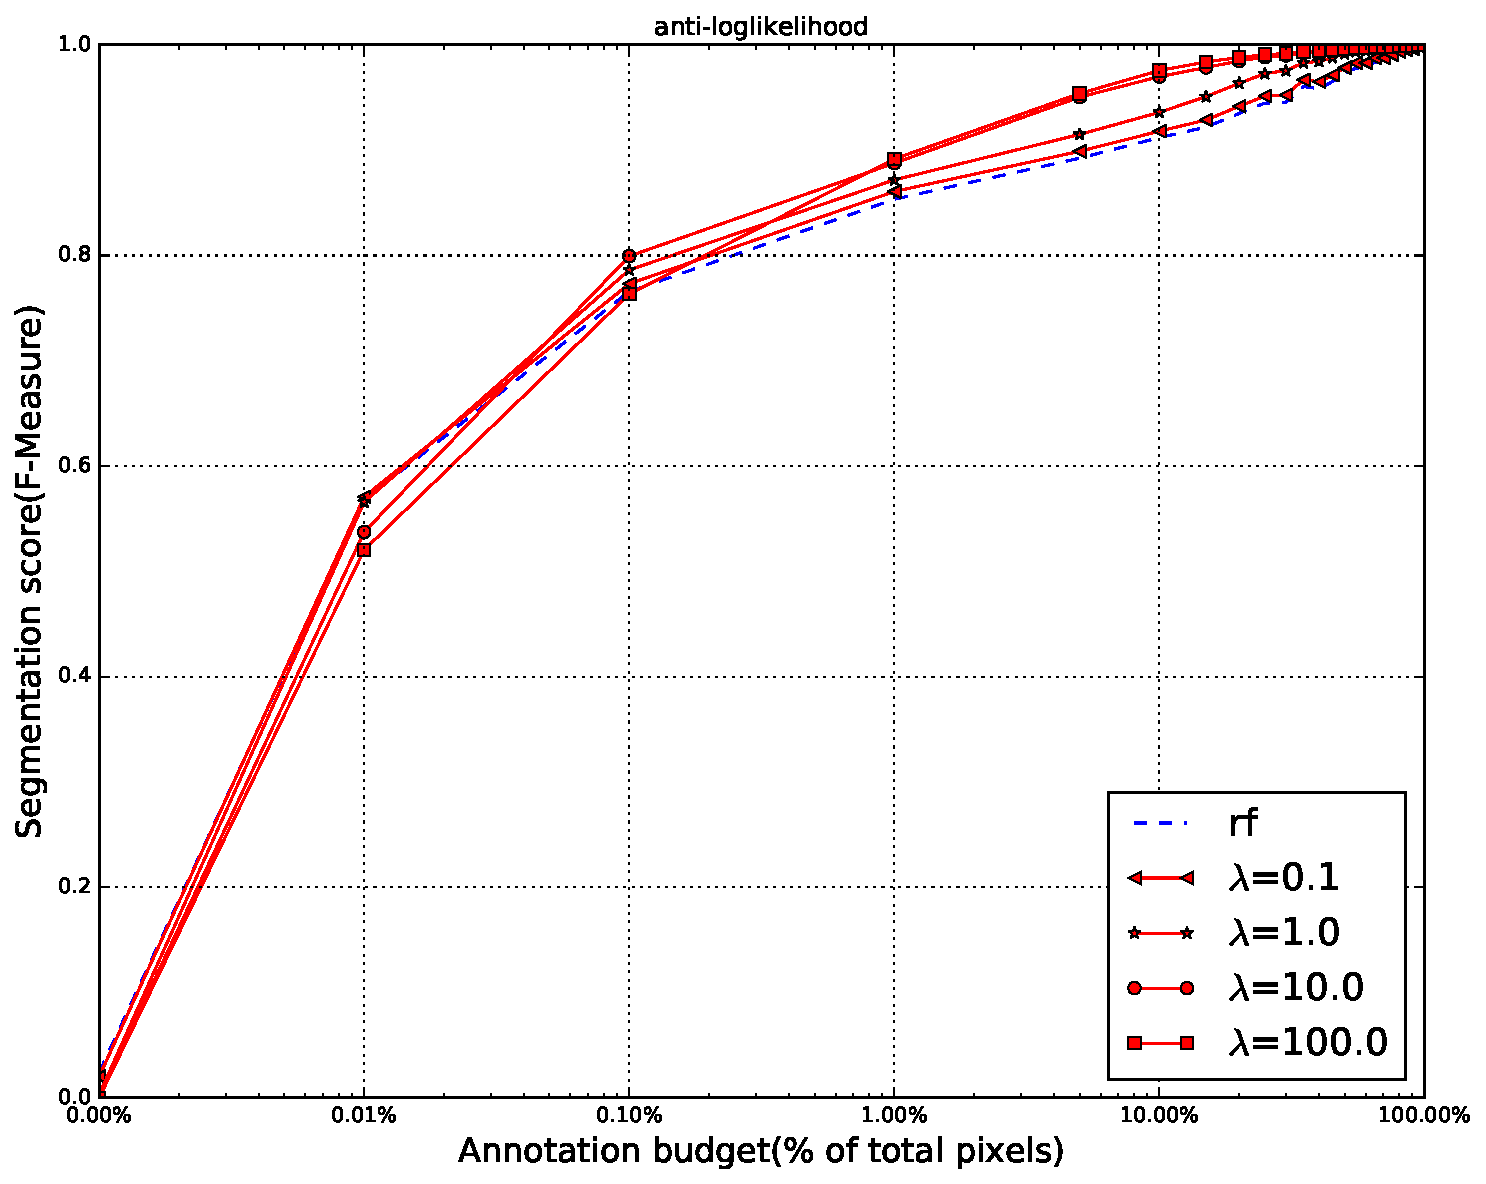
\includegraphics[width=0.8\linewidth]{figures/anti_nll.pdf}
% \end{tabular}
\caption{VIP with different cost functions}
\end{figure}

\begin{figure}[h!] \label{fig:rf_vip2}
% \begin{tabular}{ccc}
 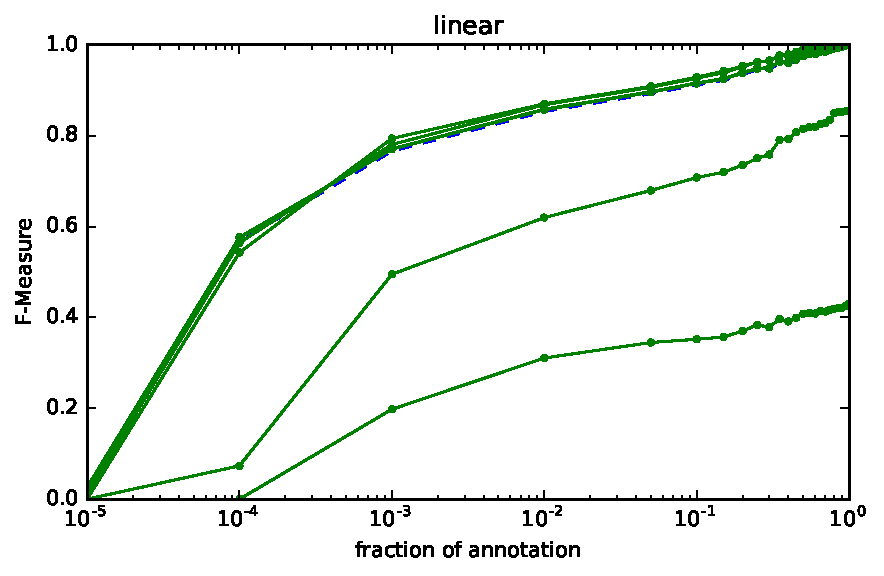
\includegraphics[width=0.8\linewidth]{figures/linear.pdf} 
% \end{tabular}
\caption{VIP with different cost functions}
\end{figure}

\begin{figure}[h!] \label{fig:rf_vip3}
% \begin{tabular}{ccc}
 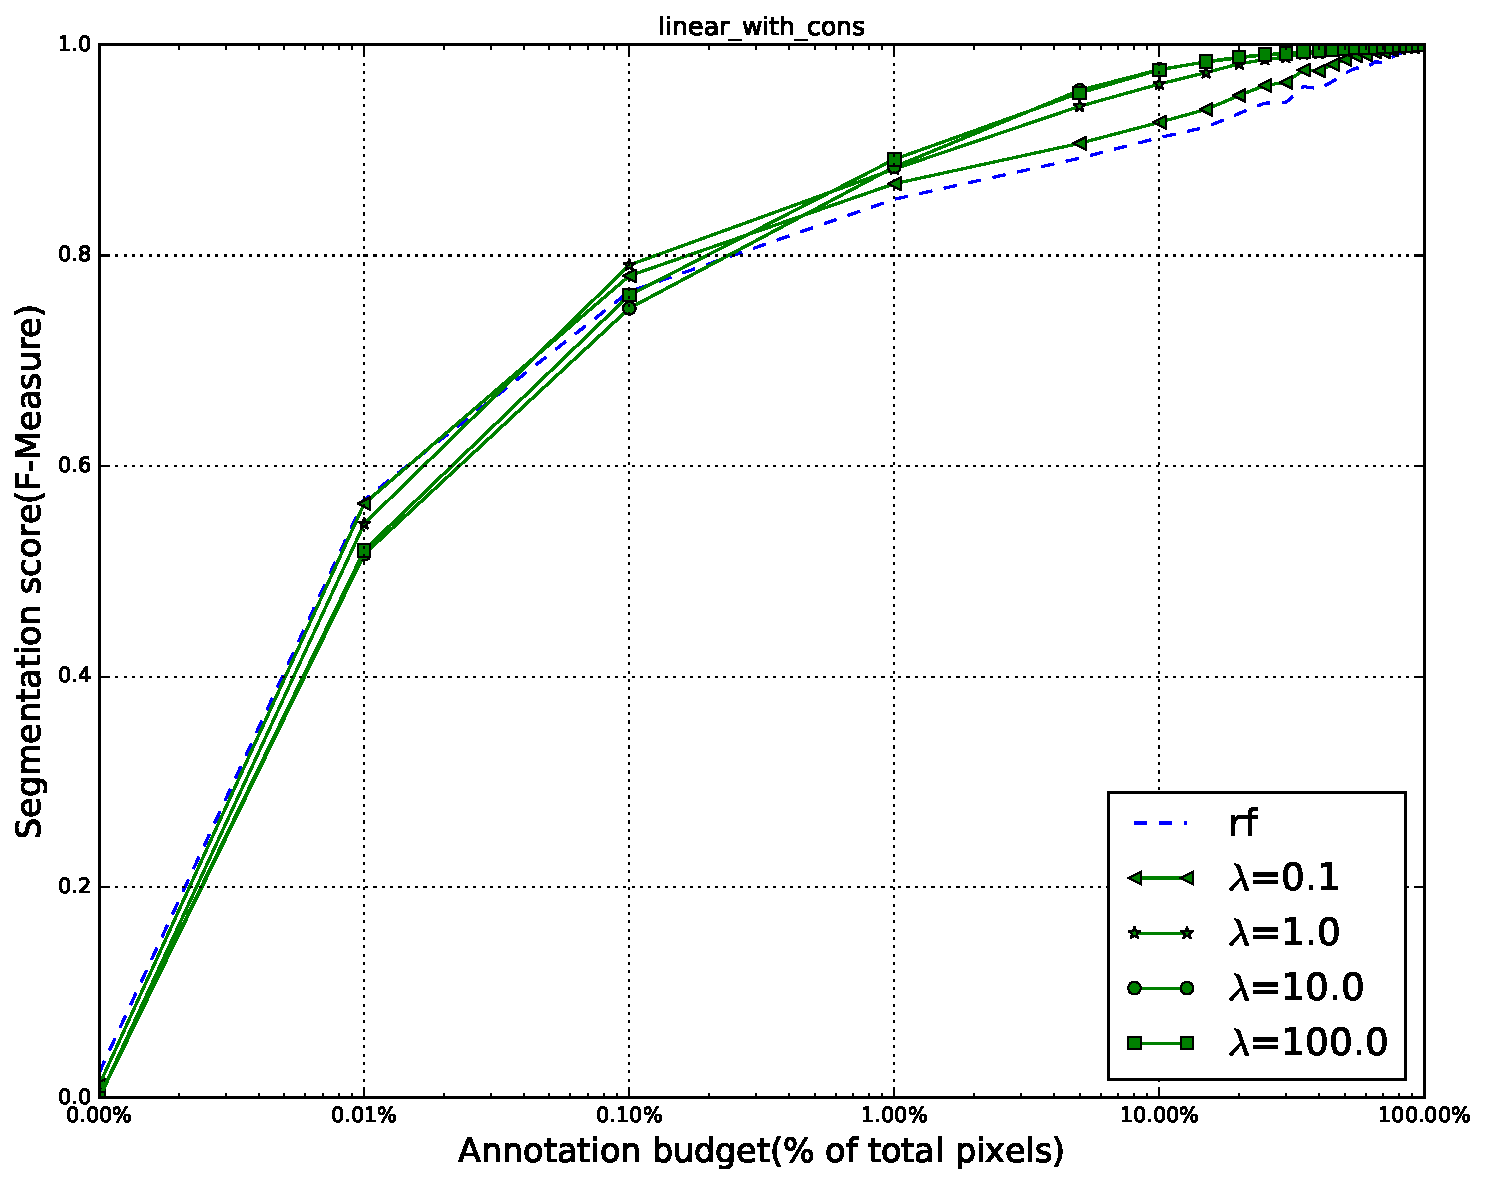
\includegraphics[width=0.8\linewidth]{figures/linear_with_cons.pdf}
% \end{tabular}
\caption{VIP with different cost functions}
\end{figure}


\begin{figure}[h!] \label{fig:rf_vip_diff}
% \begin{tabular}{ccc}
 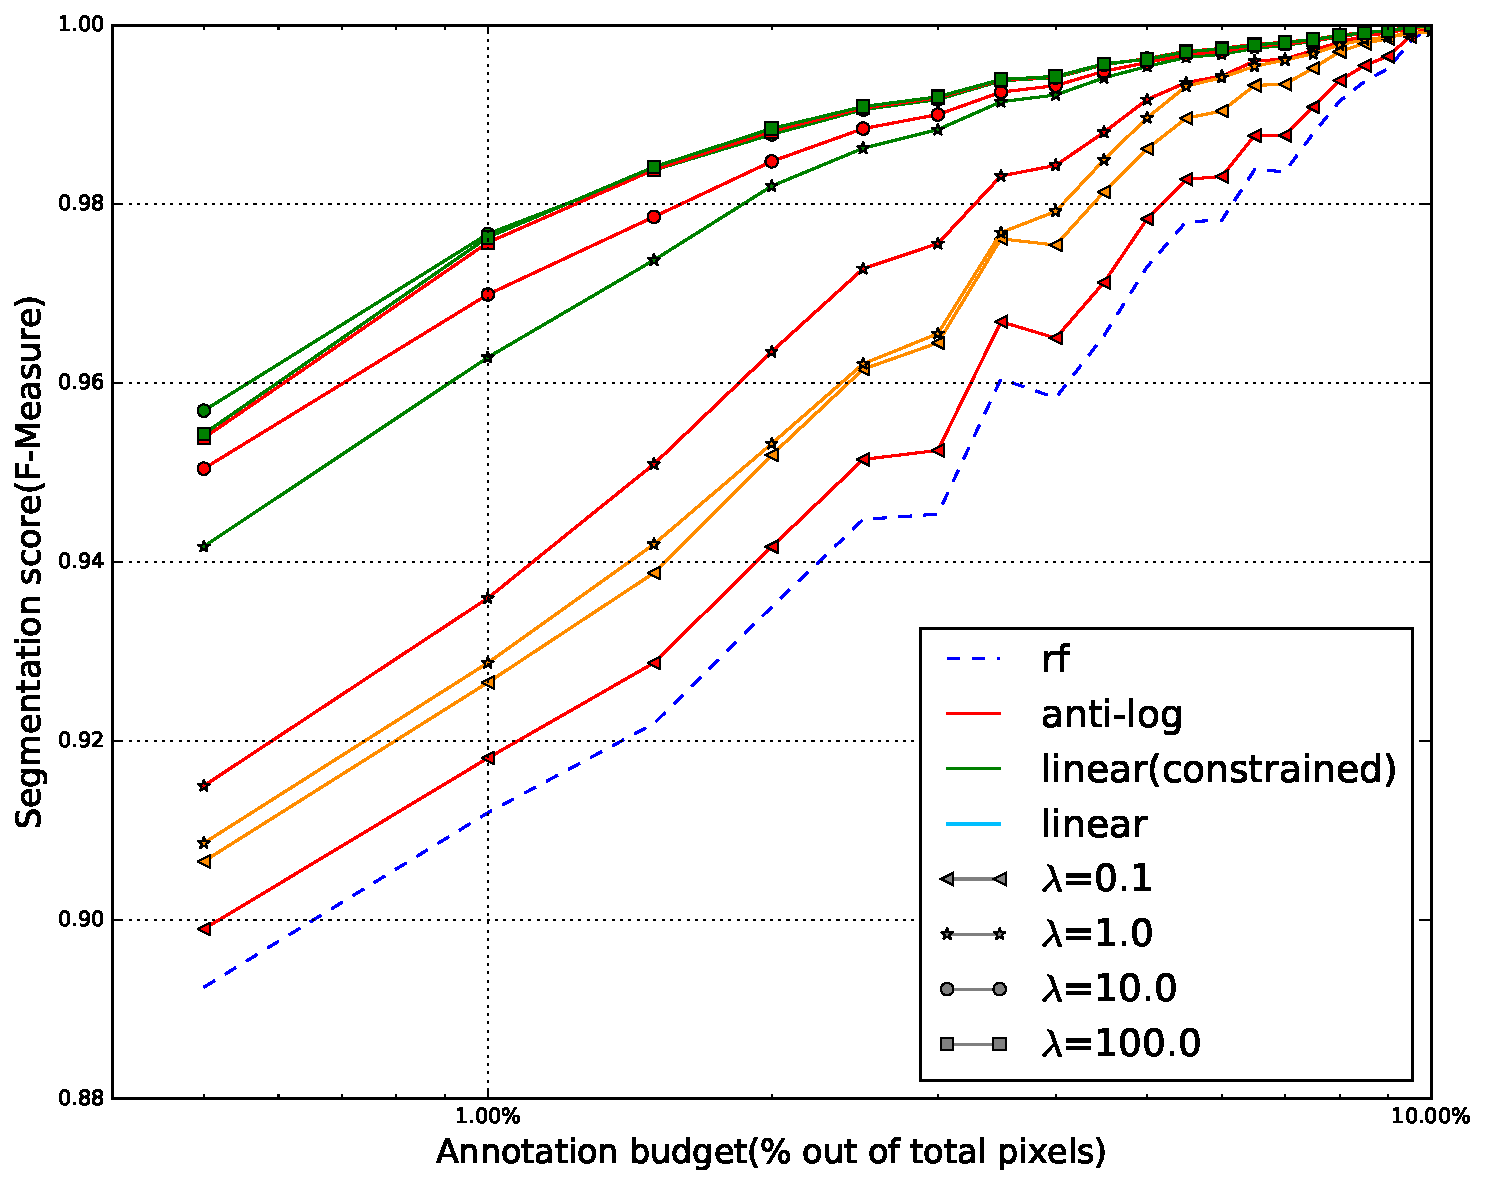
\includegraphics[width=1.0\linewidth]{figures/vip_diff.pdf}
% \end{tabular}
\caption{VIP with different cost functions}
\end{figure}


\subsection{Effect of regularisation parameter}
The use of prior information boosts up the performance but we get different boost for different value of $\lambda$. The regularisation parameter decides the weight of TV cost. One expects smooth boundaries in segmentation mask for high values, but this also effect mask for small objects. We can observe this in figure 3.9. The upper row shows that for larger vesicles, the boundary gets smooth for higher values of $\lambda$, while the bottom row shows that tiny vesicles in image tend to diminish for high values of $\lambda$. This shows that the ideal case will be to choose different $\lambda$ for different part of images or to combine results for different $\lambda$. 
% \begin{figure}[h!] \label{fig:rf_vip1}
% \begin{tabular}{ccc}
%  $\lambda=0.001$ & Ground truth & $\lambda=100.0$ \\ 
%  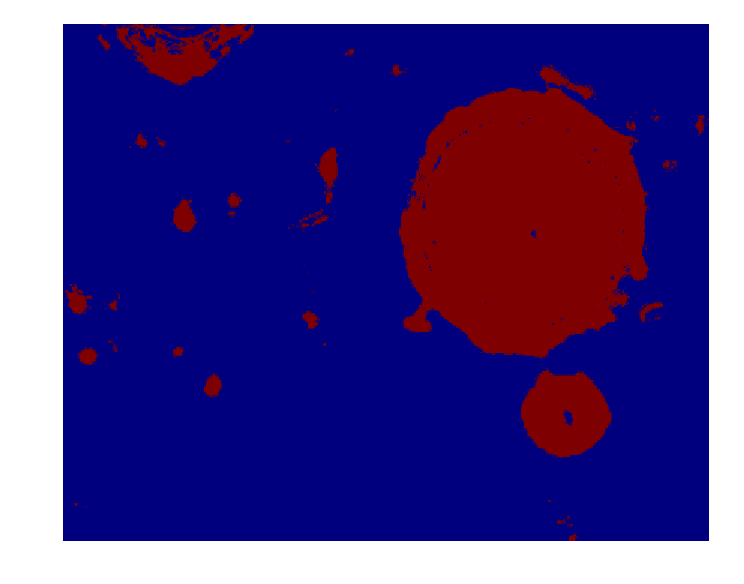
\includegraphics[width=0.33\linewidth]{figures/u_00.pdf} & 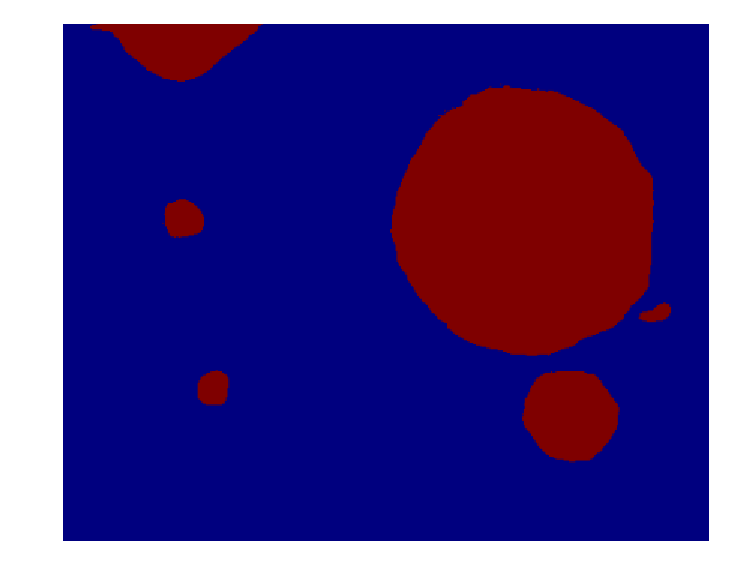
\includegraphics[width=0.33\linewidth]{figures/u_01.pdf} & 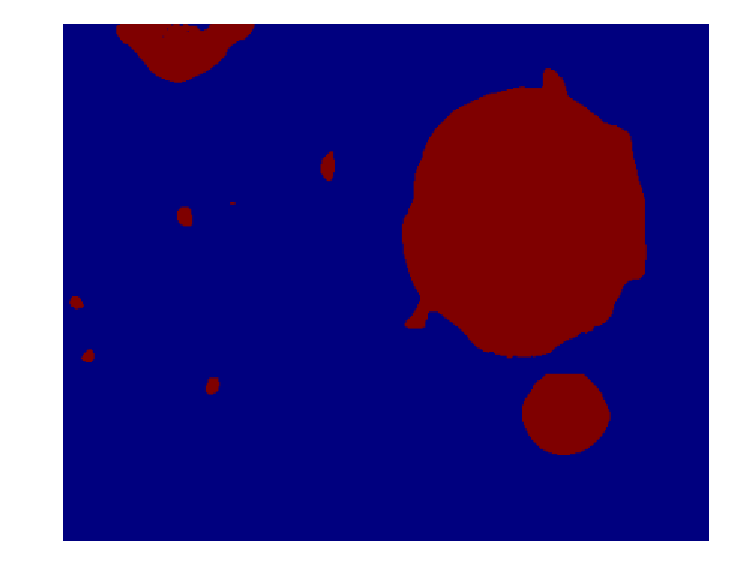
\includegraphics[width=0.33\linewidth]{figures/u_02.pdf} \\
%  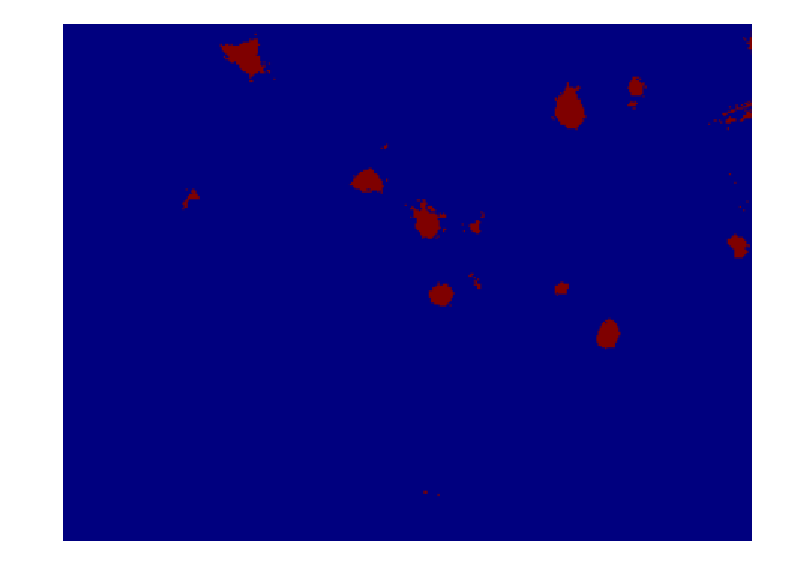
\includegraphics[width=0.33\linewidth]{figures/u_10.pdf} & 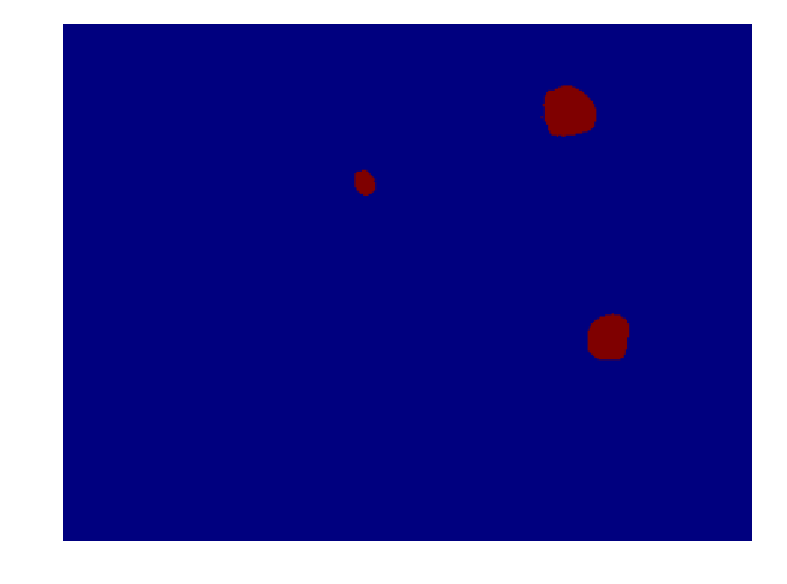
\includegraphics[width=0.33\linewidth]{figures/u_11.pdf} & 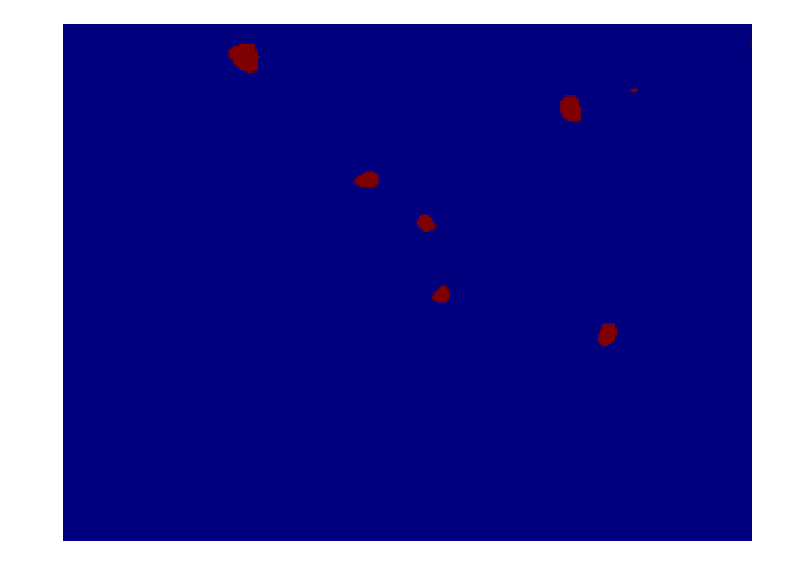
\includegraphics[width=0.33\linewidth]{figures/u_12.pdf} 
% \end{tabular}
% \caption{Segmentation mask for differnt $\lambda$ for 2 crops of image}
% \end{figure}

\begin{figure}[h!] \label{fig:effect}
 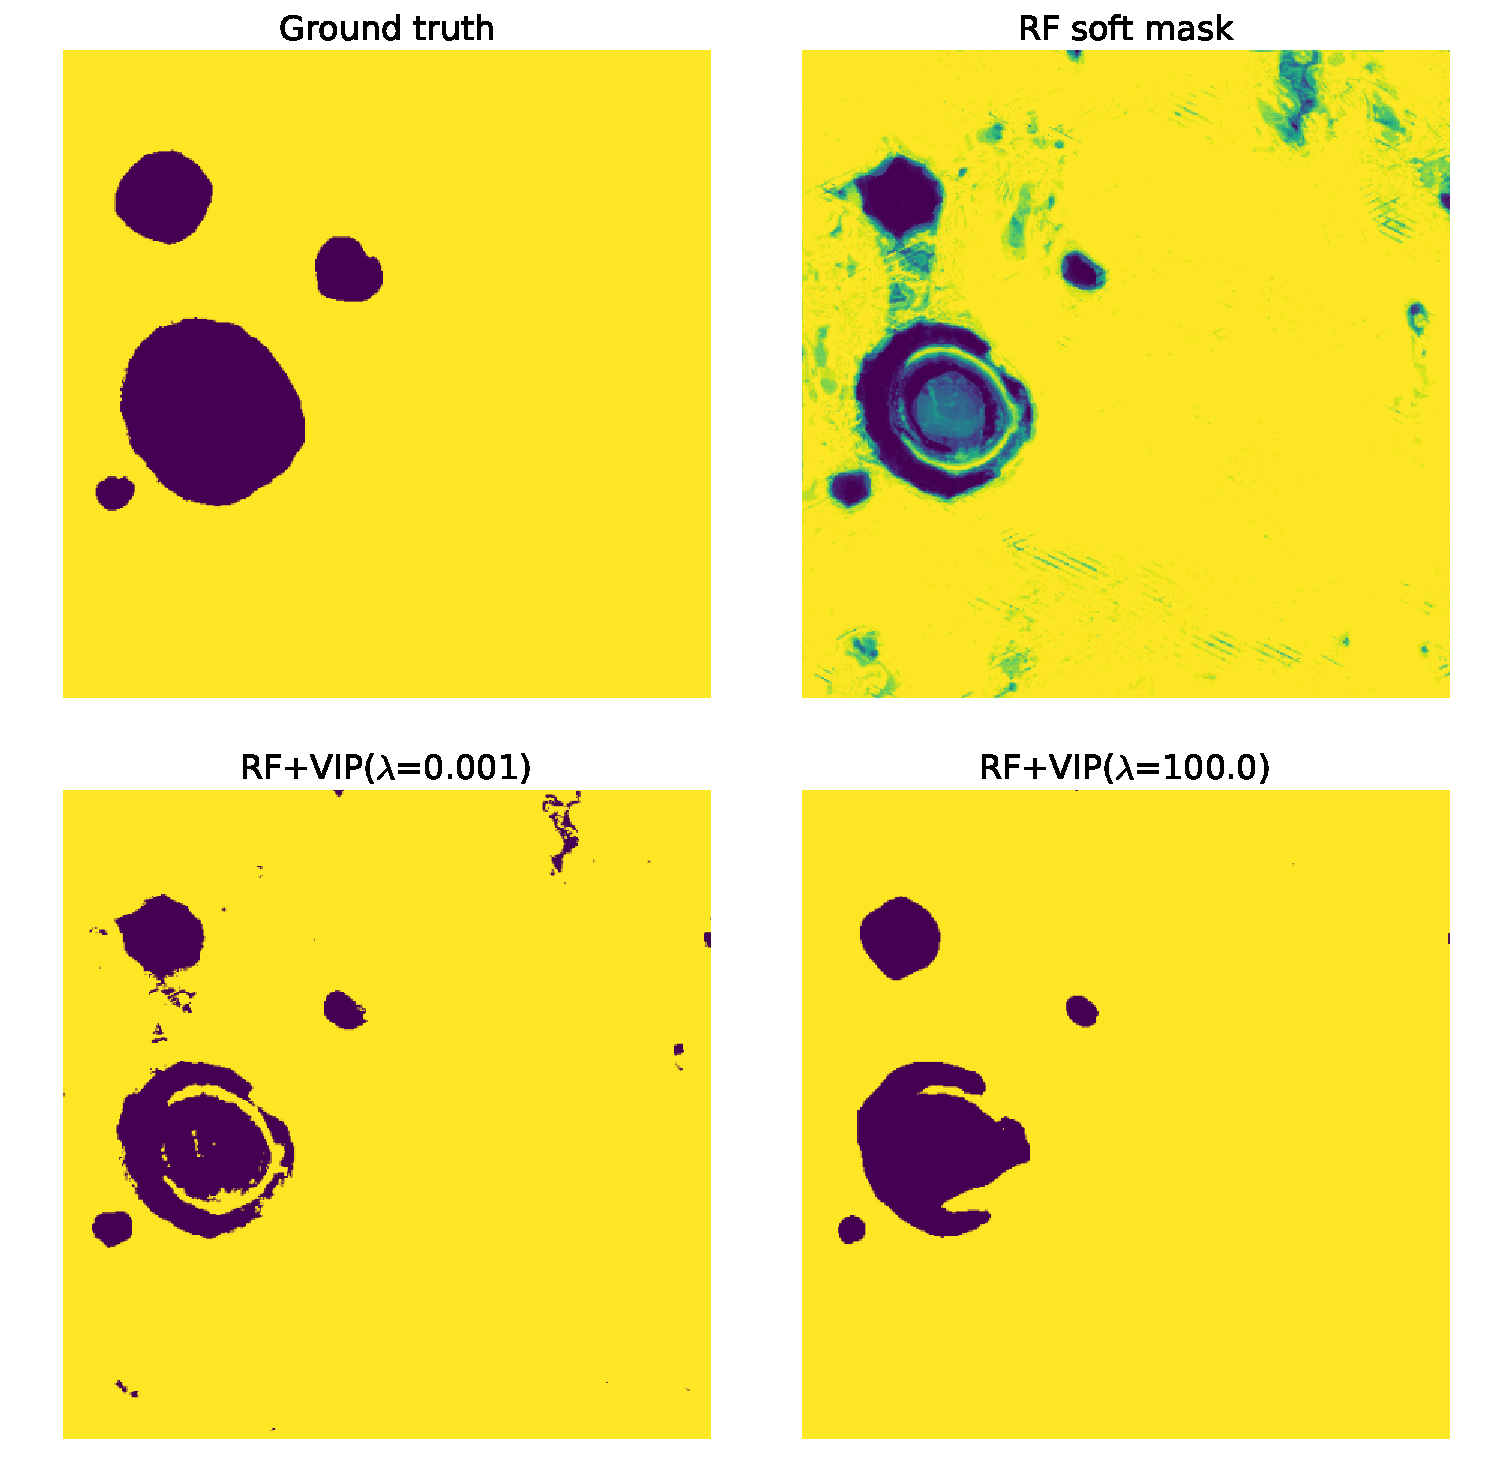
\includegraphics[width=1.0\linewidth]{figures/lamda_effect.pdf}
\caption{Segmentation mask for differnt $\lambda$ for 2 crops of image}
\end{figure}


% \subsection{2D vs 3D Total Variation}
% We observed the boost due to use to isotropic TV in 2D. Since the slices form a 3D stack, it is usual to try 3D isotropic TV. We can observe the boost in figure 3.10

\section{Semi-interactive segmentation}
We realized the need for iterative semi-interactive segmentation in section 3.1.2. With 1 iteration of interactive segmentation, we were able to improve f-measure results. Now, we combine semi-interactive annotation with the use of variational segmentation. We take segmentation mask obtained from variational segmentation and add scribbles to image where the RF and VIP together are unable to segment correctly. Then, we retrain Random forest and generate new mask using variational segmentation. The image, mask, and scribbles are shown in figure 3.10. We can observe the improvement in the mask with an addition of only 5000 pixels (less 0.2\% of pixels in the image).
\begin{figure}[h!] \label{fig:semi-vip}
 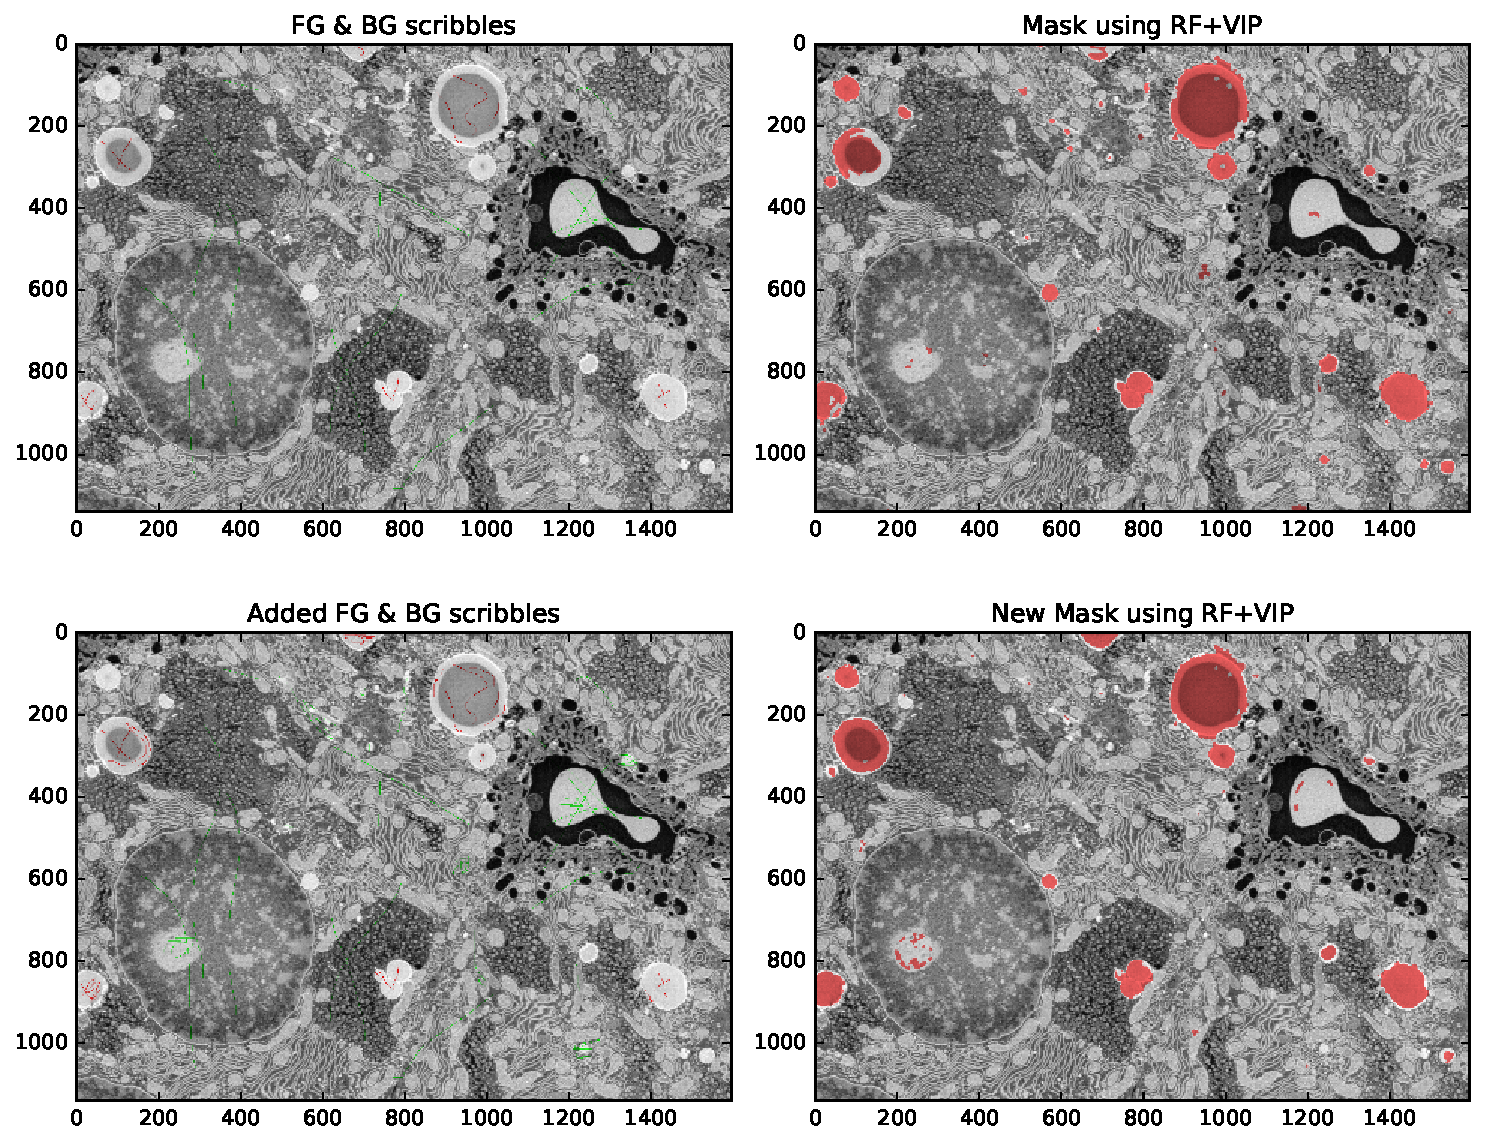
\includegraphics[width=1.0\linewidth]{figures/semi_inter_vip.pdf}
\caption{Semi-interactive segmentation with one iteration (RF+VIP)}
\end{figure}

\section{Training CNN from scribbles}
The use of Variational image processing parametrized with cost learned from RF provides a segmentation mask with good accuracy. The RF was trained with features described in WEKA toolset. These features may not work well for certain medical images and thus, use of CNN proves beneficial as it learns different feature maps according to the task. The initial layers learn basic image features while the final layers get trained for filters to compute problem specific results. In addition to this, the choice of $\lambda$ is always a problem in using VIP. As we showed in section 3.2.2, different parts of images need different values of $\lambda$ to produce best segmentation mask. Ranftl \cite{ranftl:2014} uses CNN with VIP and modifies the loss function accordingly and learns optimal values of $\lambda$ along with CNN parameters. The paper describes a method of combining CNN(5 layers) with a final variational/inference layer. The inference layer has activation function in form of Total variation. Similarly, Taylor et al. \cite{taylor:2016} implemented CNN as a scalable ADMM approach. They split the objective function into subproblems (as we did using ASB) and trained CNN without gradients. These papers attempt to couple CNN with VIP to gain from both approaches. \par

This motivated us to replace RF with CNN to parametrize cost function. In literature, we can find multiple approaches to train CNN using scribbles. Gonda et al.\cite{Gonda:2016} uses an interactive approach to train deep neural networks for segmentation of neuronal structures using scribbles. Lai et al. \cite{Lai:2015} uses patch-based 3D image segmentation. They make use of patches around pixels annotated to train the neural network. A similar approach has been used by Havaei et al.\cite{Havaei:2015} for brain tumor segmentation using deep neural networks. These ideas take each pixel as a sample and CNN is trained as a classifier to classify each pixel. The disadvantage is that we remove one major property of CNN to adapt its final layers according to full image for segmentation task and also, it needs sufficient data to train CNN. Therefore, we tried to train OSVOS network (explained in Section 2) from scribbles using \textbf{cross entropy scribble loss}. The simple trick we used was to replace computation of cross-entropy loss function for the complete image by computing loss for only annotated scribbles. The \textbf{cross entropy scribble loss} can be computed at each pixel, $x$ with probability $p$, as defined below:

\begin{align*}
\funop{l_{scribble}}(x) =
\begin{cases}
  -z(x)\,log(p(x)) - (1 - z(x))\,log(1 - p(x)), & \text{if}\ x \in \text{Scribbles}  \\
  0, & \text{else}
\end{cases}
\end{align*}

We succeeded in training our network with scribble loss and results can be seen in figure 3.11. We compared the results obtained for both RF and CNN using the same amount of pixels annotated. It can be observed that RF looks to perform better for a lower amount of scribbles, while CNN reaches f-measure of a maximum of 0.86 for higher annotation budget.
The mask generated using CNN from scribbles shows uncertainity for pixels at boundaries. Thus, we used Variational image processing over mask obtained from CNN. The boost with VIP can be observed in figure 3.12.
\begin{figure}[h!] \label{fig:cnnvip}
 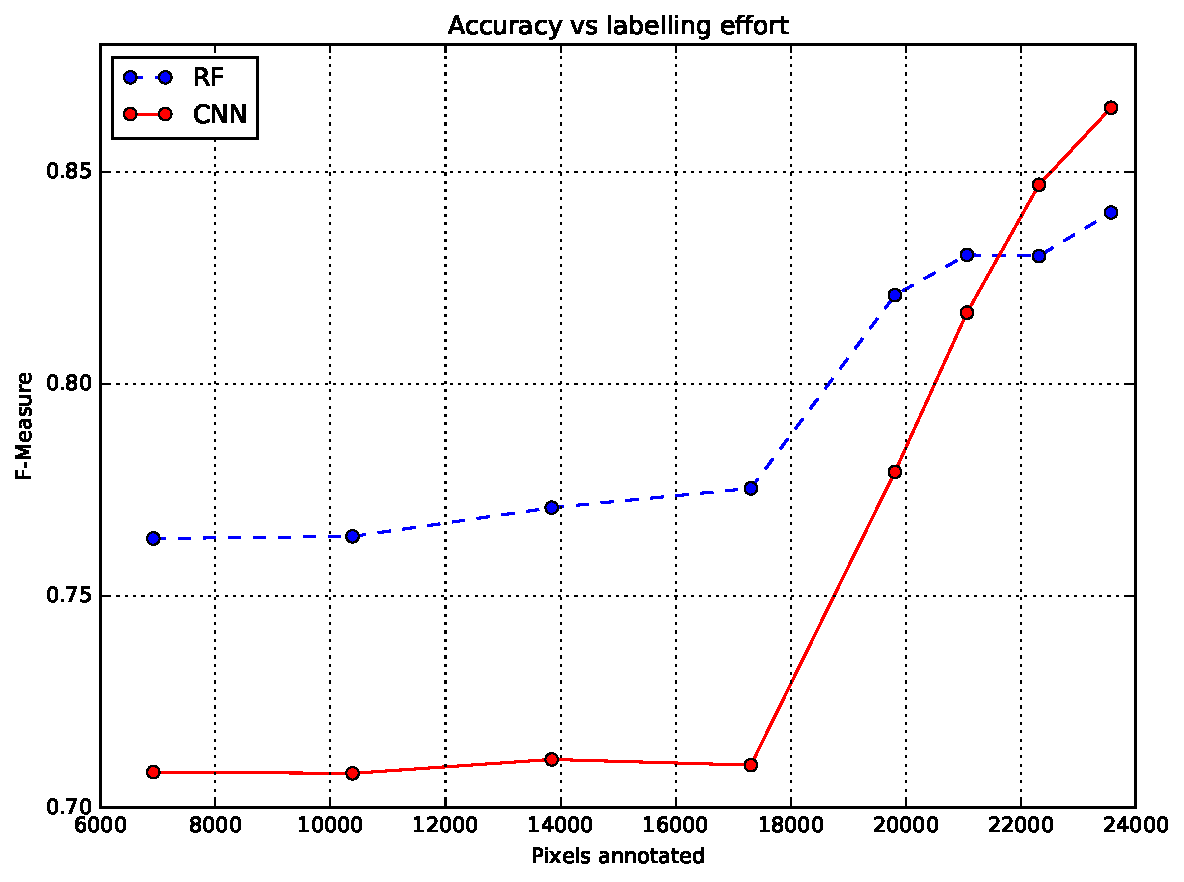
\includegraphics[width=1.0\linewidth]{figures/cnn_vs_rf.pdf} 
\caption{F-measure for increasing annotation budget for comparing CNN vs RF}
\end{figure}

\begin{figure}[h!] \label{fig:cnnvip}
 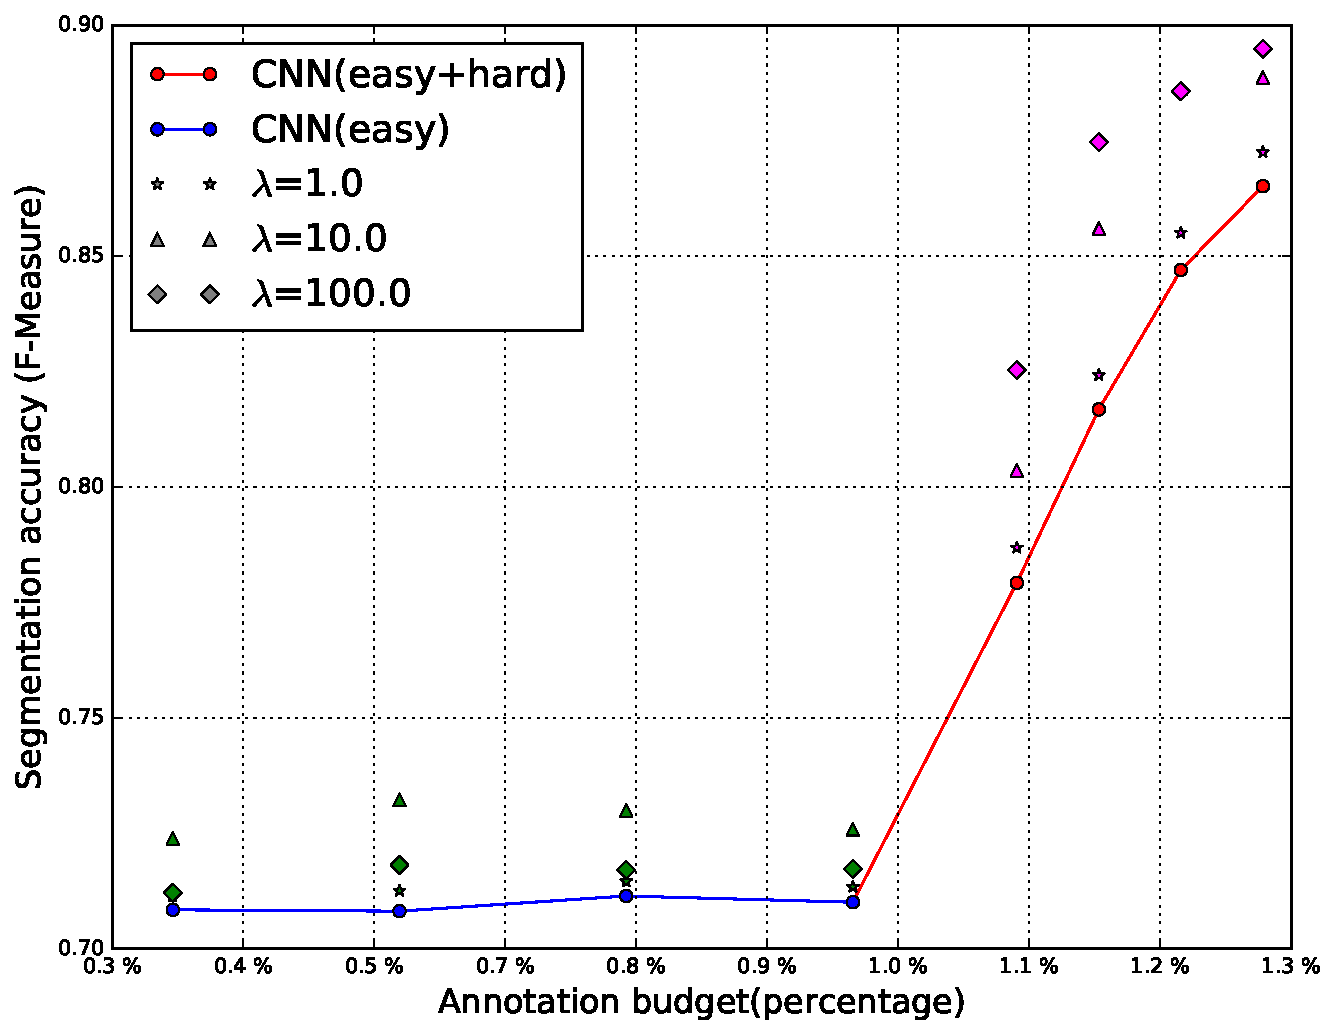
\includegraphics[width=0.8\linewidth]{figures/cnn_vip.pdf}
 \caption{(a) CNN with VIP (different $\lambda$)\, (b) CNN vs RF with VIP}
\end{figure}


\begin{figure}[h!] \label{fig:cnnvip}
 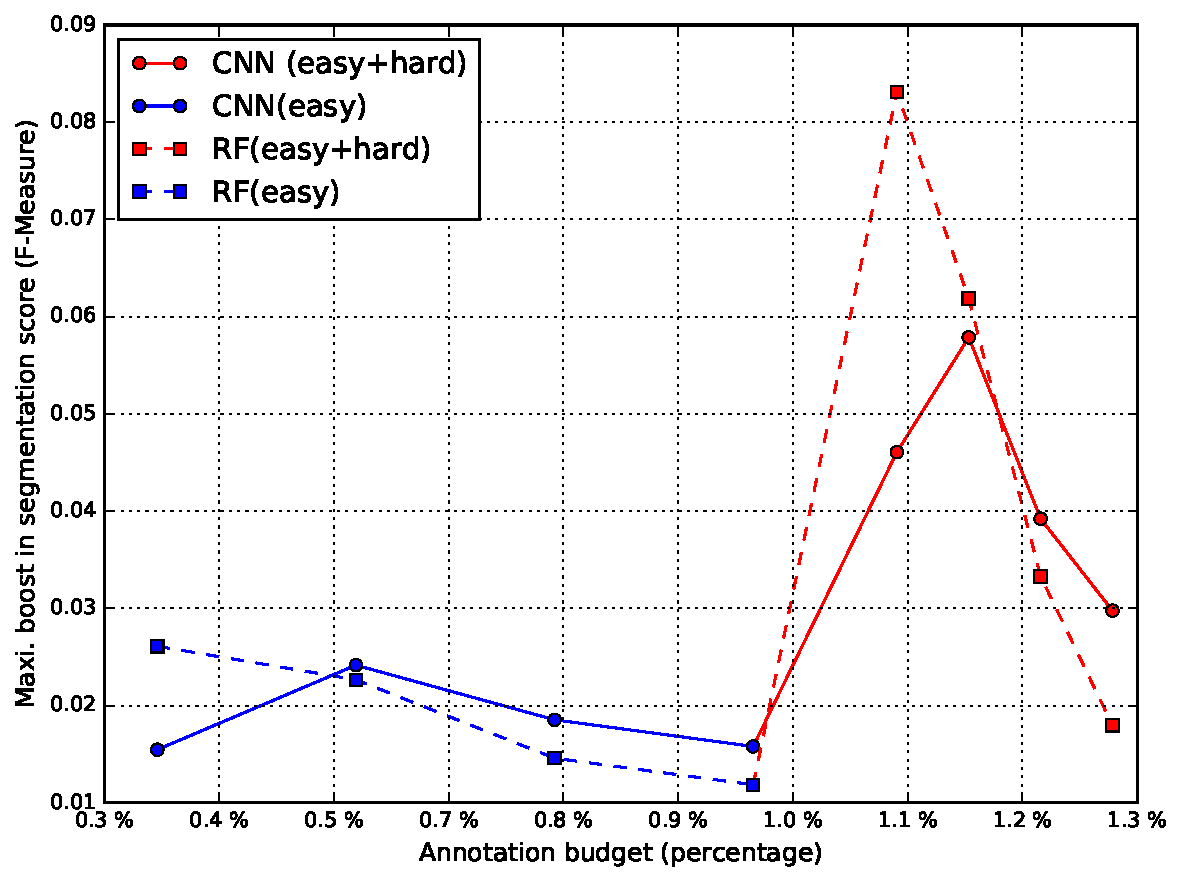
\includegraphics[width=0.8\linewidth]{figures/cnn_vip_boost.pdf}
\caption{(a) CNN with VIP (different $\lambda$)\, (b) CNN vs RF with VIP}
\end{figure}


\begin{figure}[h!] \label{fig:cnnvip}
 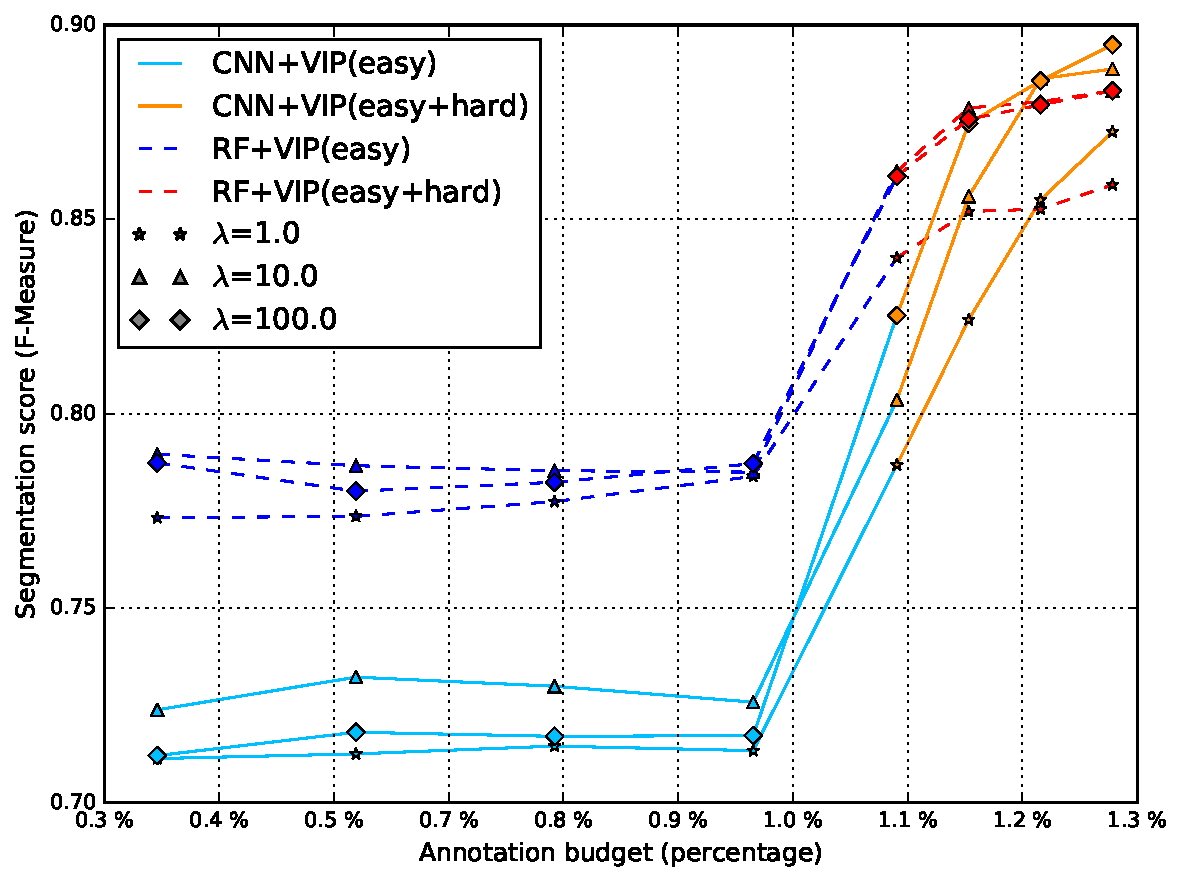
\includegraphics[width=0.8\linewidth]{figures/cnn_vs_rf_vip.pdf} 
\caption{(a) CNN with VIP (different $\lambda$)\, (b) CNN vs RF with VIP}
\end{figure}